%!TEX root = Manuscript.tex

\chapter{Result of precise matching}
\label{chap:appendixB}




\begin{figure*}[htbp]
	\begin{center}
		\subfigure[Common zone]{
			\begin{minipage}[t]{0.48\linewidth}
				\centering
				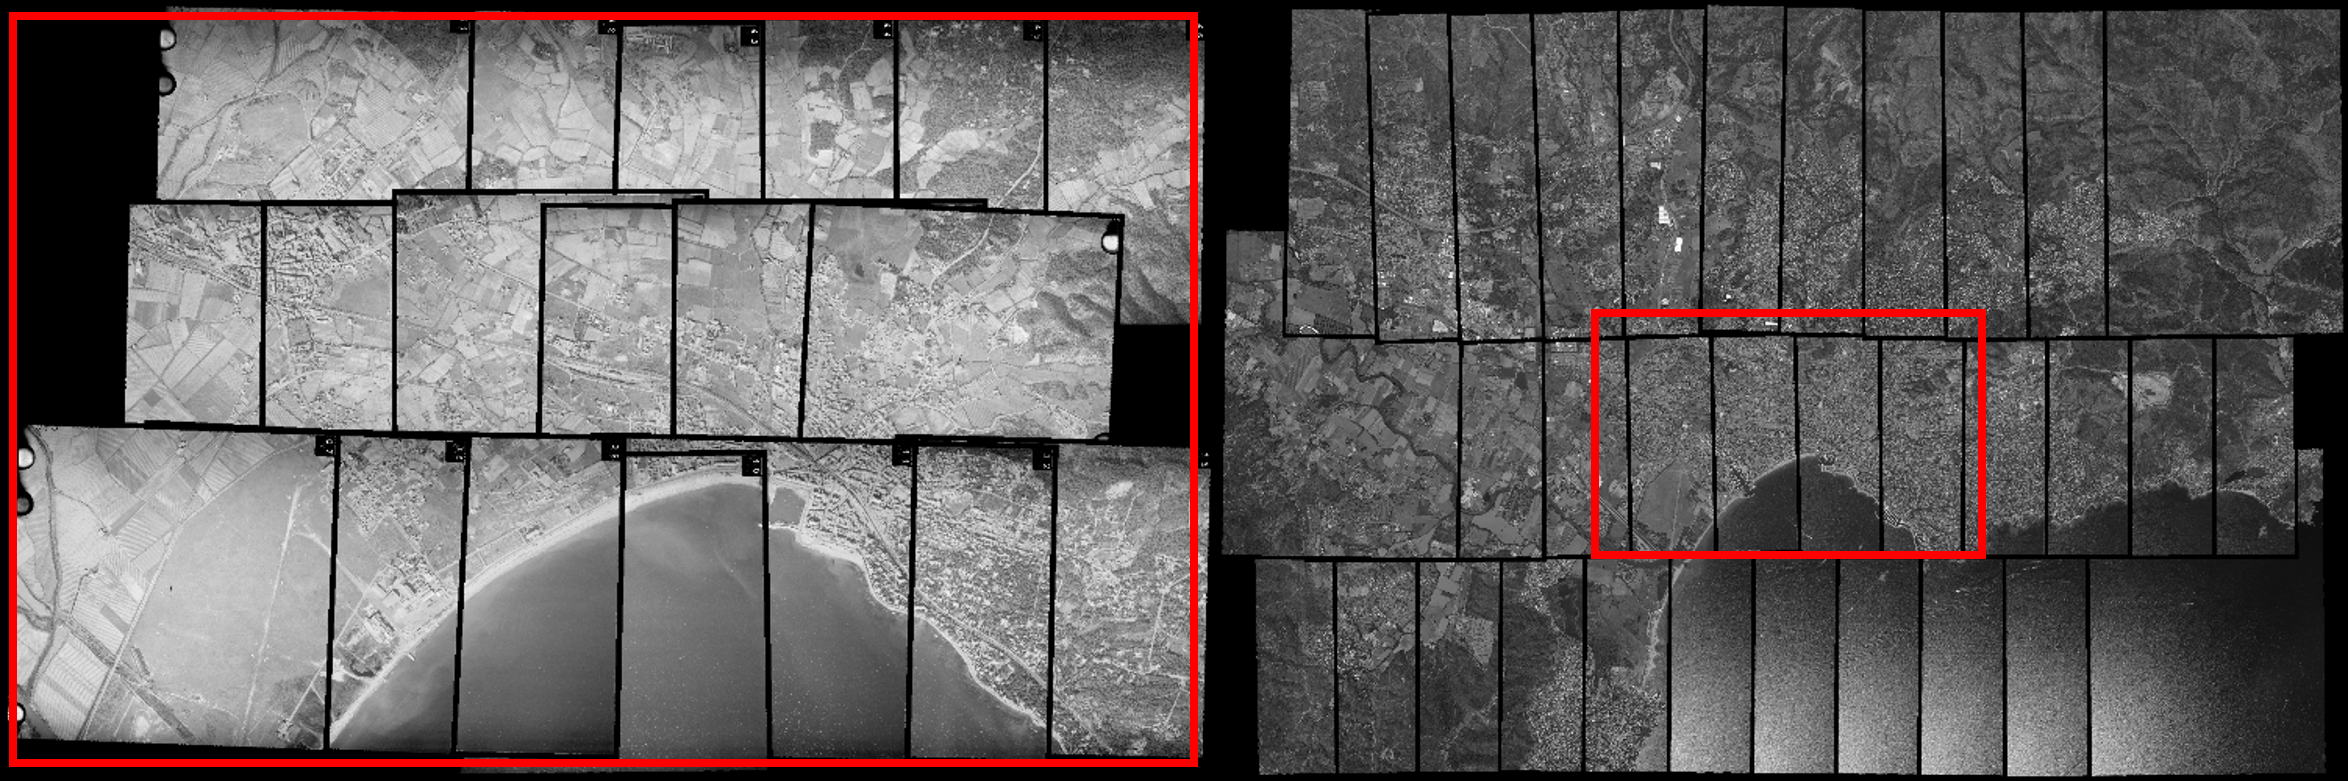
\includegraphics[width=6.8cm]{images/Chapitre3/Pseudo-Ortho-MEC-Malt_Tapas_1954_Ortho-MEC-Malt_2014.png}
			\end{minipage}%
		}
		\subfigure[Number of recovered matches]{
			\begin{minipage}[t]{0.48\linewidth}
				\centering
				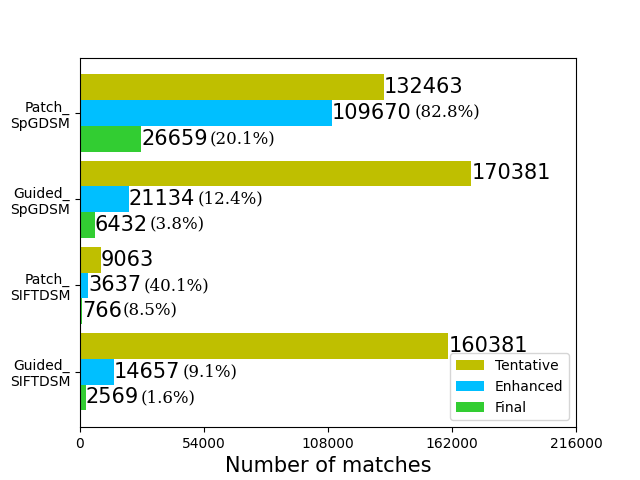
\includegraphics[width=5.8cm]{images/Chapitre4/PlotBarH-Frejus1954-2014.png}
			\end{minipage}%
		}
		\subfigure[$Patch_{SpGDSM}$]{
			\begin{minipage}[t]{0.48\linewidth}
				\centering
				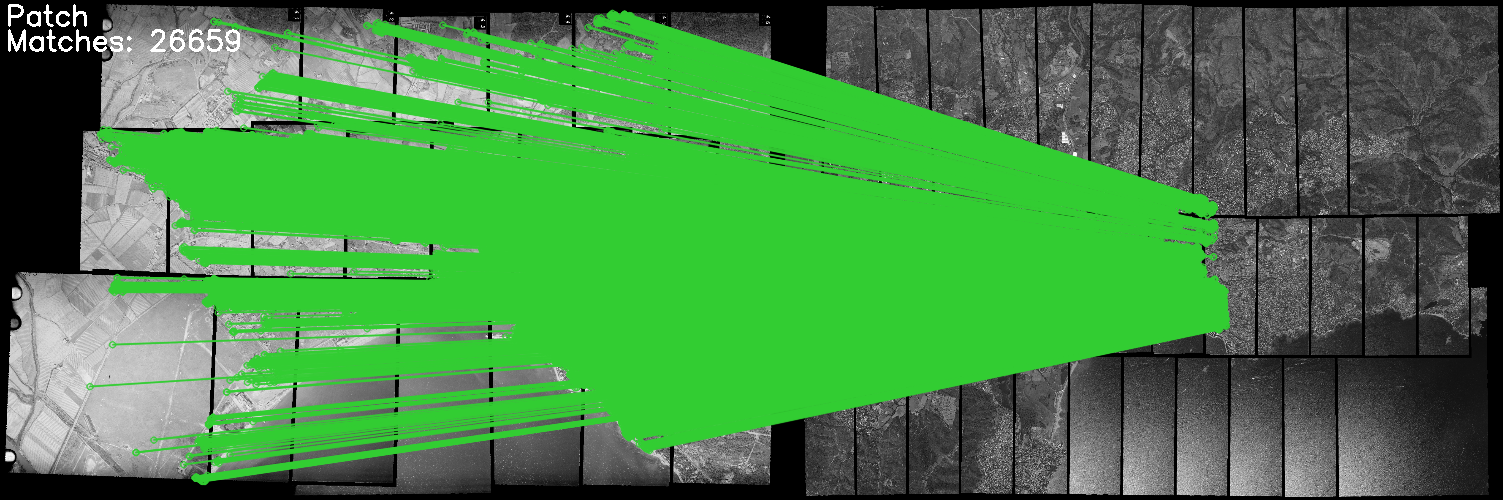
\includegraphics[width=6.8cm]{images/Chapitre4/Precise-SpGDSMHomol-1954-2014-SuperGlue-3DRANSAC-CrossCorrelation-PileImg_Ortho-MEC-Malt_Tapas_1954_Ortho-MEC-Malt_2014.png}
			\end{minipage}%
		}
		\subfigure[$Guided_{SpGDSM}$]{
			\begin{minipage}[t]{0.48\linewidth}
				\centering
				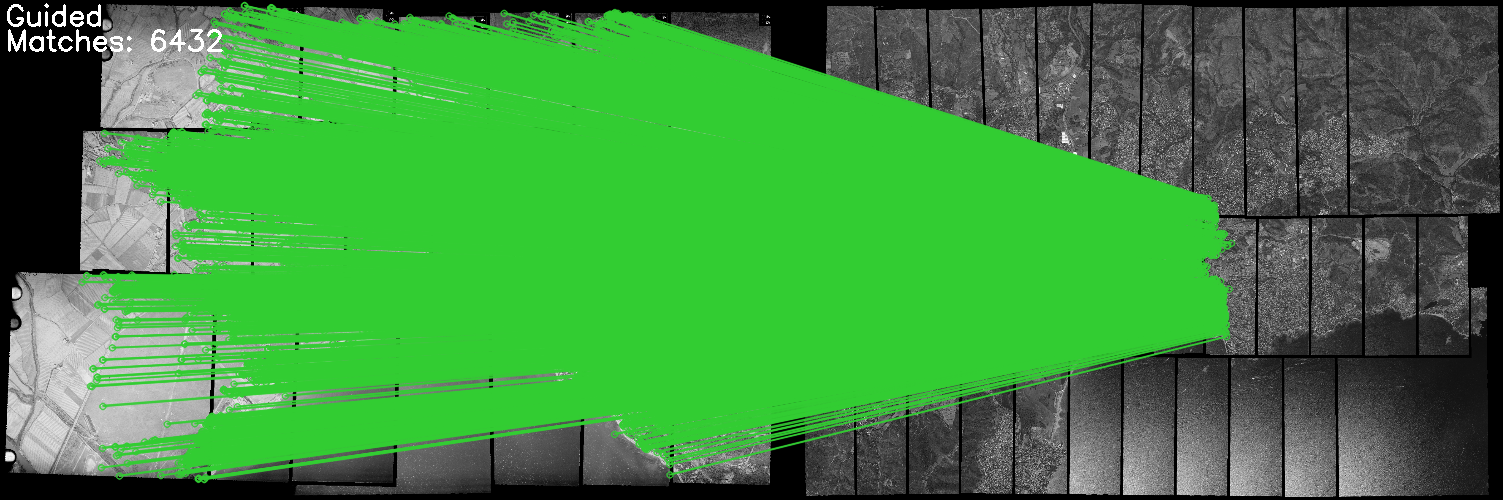
\includegraphics[width=6.8cm]{images/Chapitre4/Precise-SpGDSMHomol-1954-2014-GuidedSIFT-3DRANSAC-CrossCorrelation-PileImg_Ortho-MEC-Malt_Tapas_1954_Ortho-MEC-Malt_2014.png}
			\end{minipage}%
		}
		\subfigure[$Patch_{SIFTDSM}$]{
			\begin{minipage}[t]{0.48\linewidth}
				\centering
				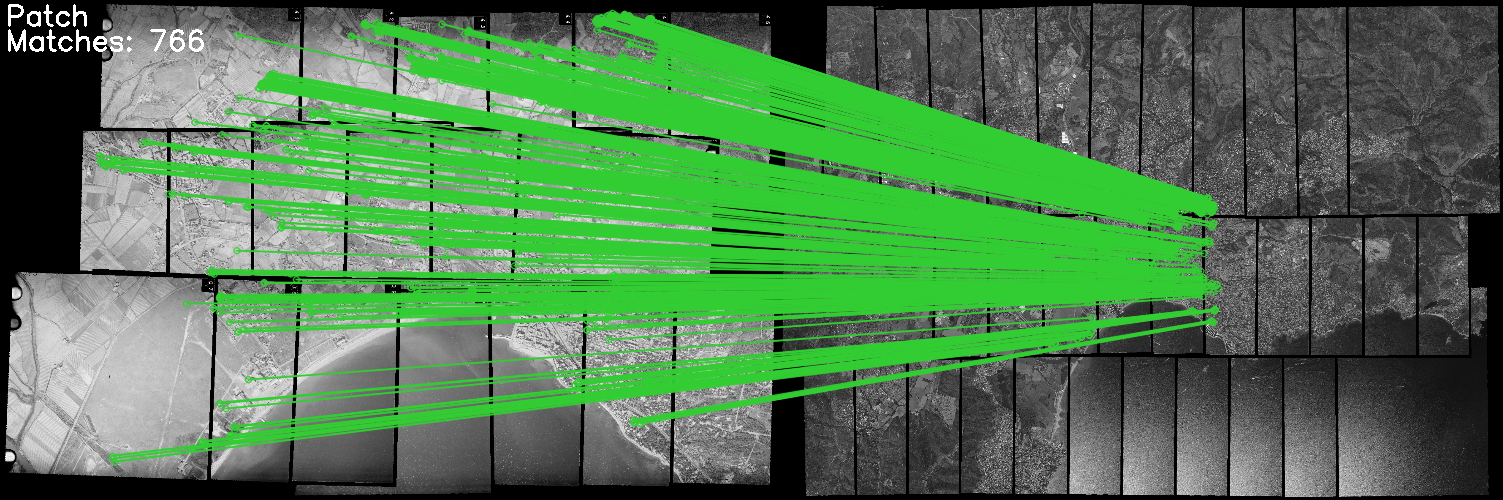
\includegraphics[width=6.8cm]{images/Chapitre4/Precise-SIFTDSMHomol-1954-2014-SuperGlue-3DRANSAC-CrossCorrelation-PileImg_Ortho-MEC-Malt_Tapas_1954_Ortho-MEC-Malt_2014.png}
			\end{minipage}%
		}
		\subfigure[$Guided_{SIFTDSM}$]{
			\begin{minipage}[t]{0.48\linewidth}
				\centering
				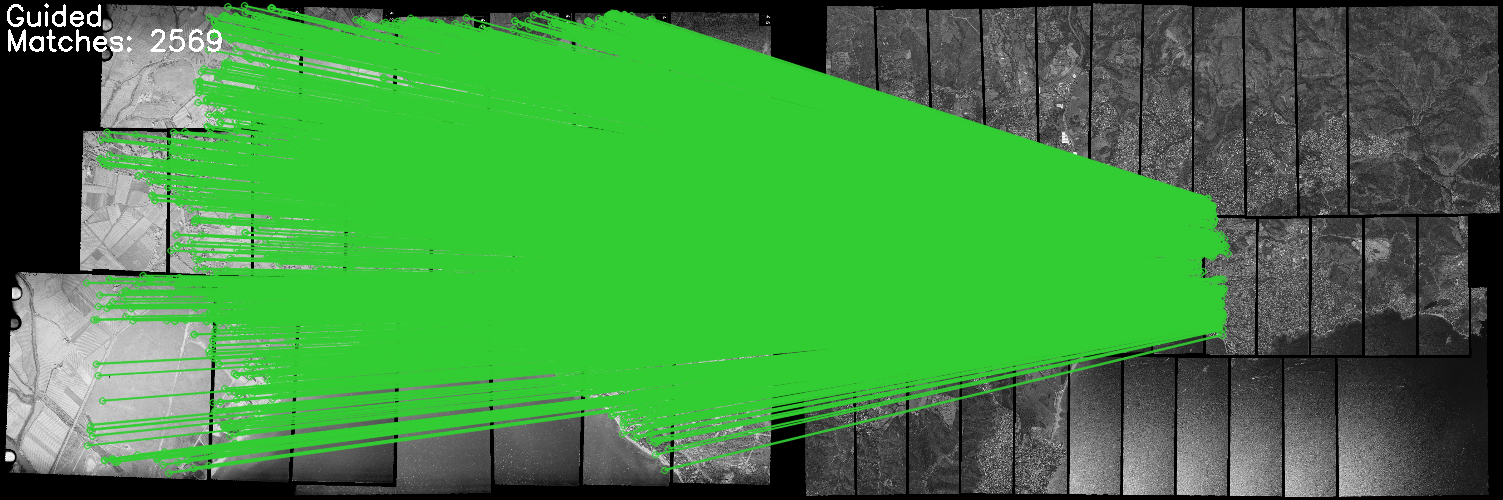
\includegraphics[width=6.8cm]{images/Chapitre4/Precise-SIFTDSMHomol-1954-2014-GuidedSIFT-3DRANSAC-CrossCorrelation-PileImg_Ortho-MEC-Malt_Tapas_1954_Ortho-MEC-Malt_2014.png}
			\end{minipage}%
		}
		\caption{Precise matching visualization of \textbf{Fr{\'e}jus 1954 and 2014}. (a) Image pairs to be matched, with red rectangles indicating the common zone. (b) Numbers of tentative, enhanced and final matches recovered with $Patch_{SpGDSM}$, $Guided_{SpGDSM}$, $Patch_{SIFTDSM}$ and $Guided_{SIFTDSM}$ individually. (c-f) Visualization of final matches recovered with $Patch_{SpGDSM}$, $Guided_{SpGDSM}$, $Patch_{SIFTDSM}$ and $Guided_{SIFTDSM}$ individually.}
		\label{MatchVizFrejus1954-2014}
	\end{center}
\end{figure*} 


\begin{figure*}[htbp]
	\begin{center}
		\subfigure[Common zone]{
			\begin{minipage}[t]{0.48\linewidth}
				\centering
				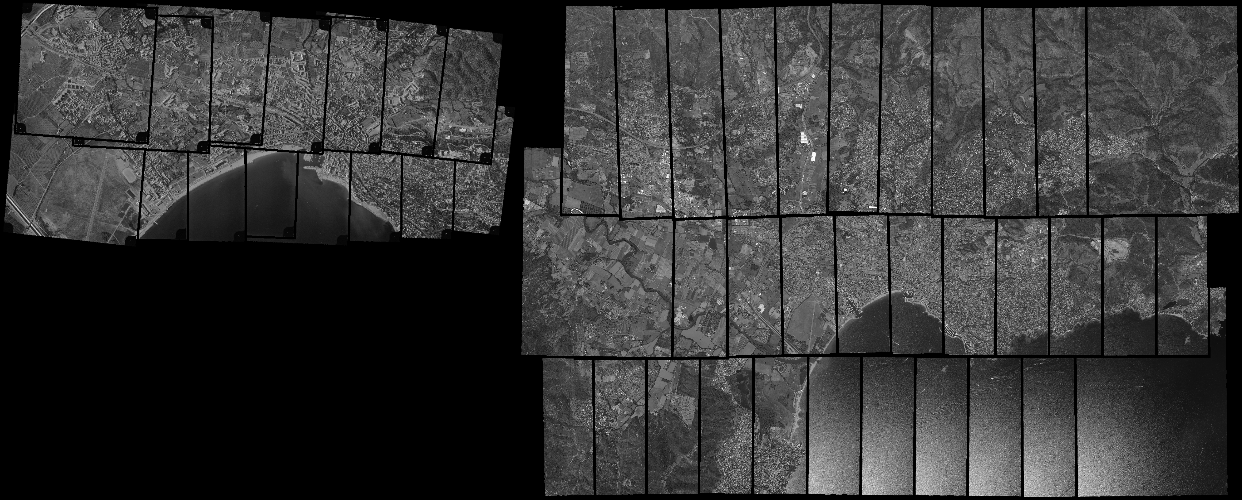
\includegraphics[width=6.8cm]{images/Chapitre3/Pseudo-Ortho-MEC-Malt_Tapas_1966_Ortho-MEC-Malt_2014.png}
			\end{minipage}%
		}
		\subfigure[Number of recovered matches]{
			\begin{minipage}[t]{0.48\linewidth}
				\centering
				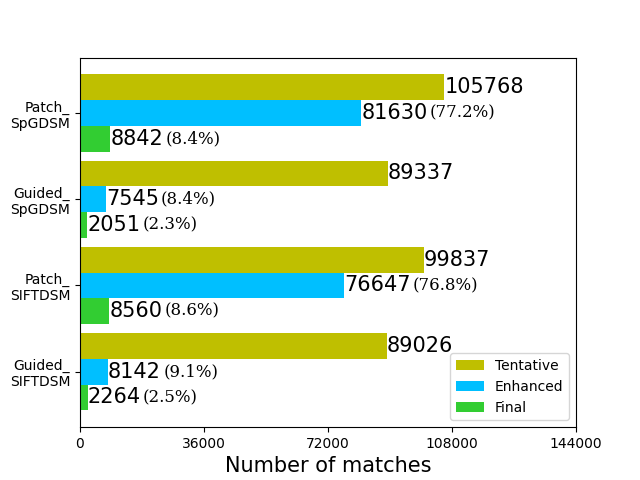
\includegraphics[width=5.8cm]{images/Chapitre4/PlotBarH-Frejus1966-2014.png}
			\end{minipage}%
		}
		\subfigure[$Patch_{SpGDSM}$]{
			\begin{minipage}[t]{0.48\linewidth}
				\centering
				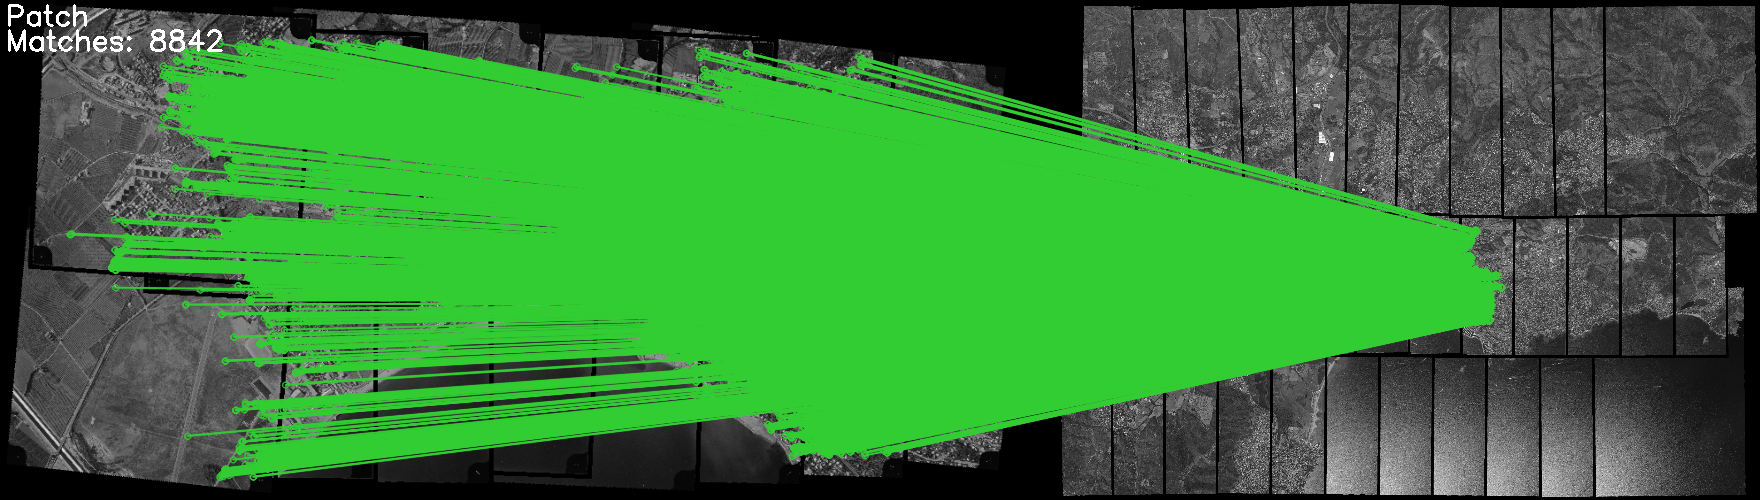
\includegraphics[width=6.8cm]{images/Chapitre4/Precise-SpGDSMHomol-1966-2014-SuperGlue-3DRANSAC-CrossCorrelation-PileImg_Ortho-MEC-Malt_Tapas_1966_Ortho-MEC-Malt_2014.png}
			\end{minipage}%
		}
		\subfigure[$Guided_{SpGDSM}$]{
			\begin{minipage}[t]{0.48\linewidth}
				\centering
				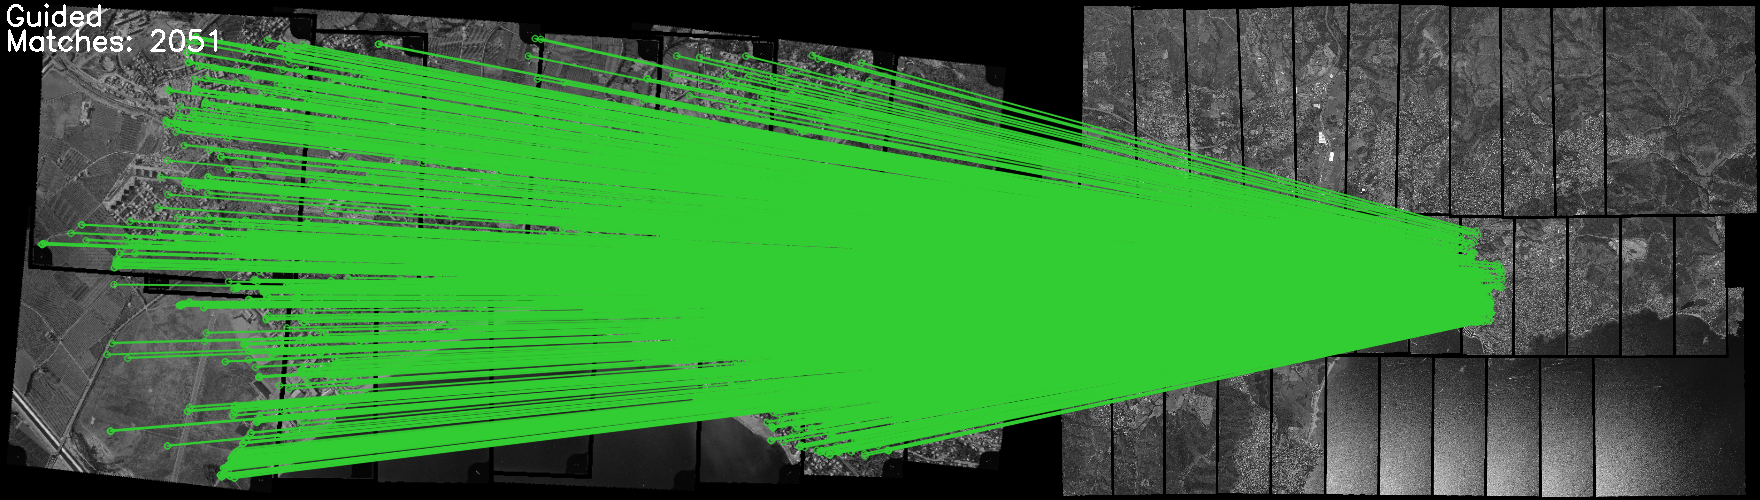
\includegraphics[width=6.8cm]{images/Chapitre4/Precise-SpGDSMHomol-1966-2014-GuidedSIFT-3DRANSAC-CrossCorrelation-PileImg_Ortho-MEC-Malt_Tapas_1966_Ortho-MEC-Malt_2014.png}
			\end{minipage}%
		}
		\subfigure[$Patch_{SIFTDSM}$]{
			\begin{minipage}[t]{0.48\linewidth}
				\centering
				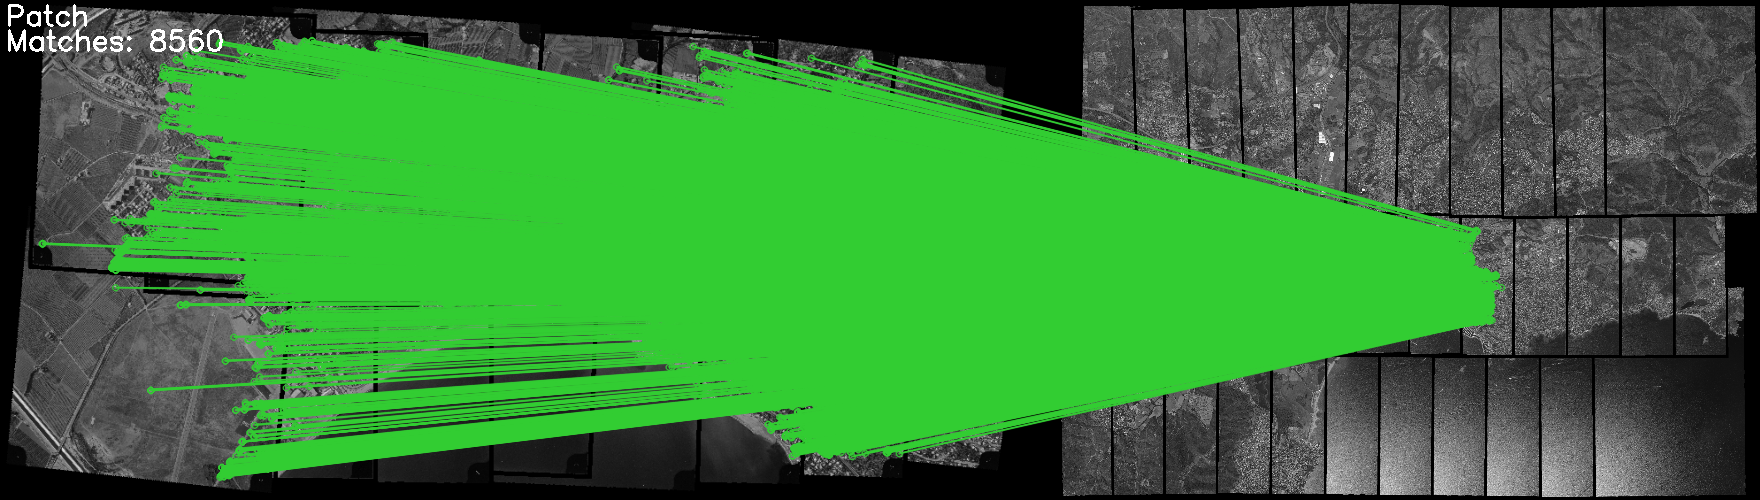
\includegraphics[width=6.8cm]{images/Chapitre4/Precise-SIFTDSMHomol-1966-2014-SuperGlue-3DRANSAC-CrossCorrelation-PileImg_Ortho-MEC-Malt_Tapas_1966_Ortho-MEC-Malt_2014.png}
			\end{minipage}%
		}
		\subfigure[$Guided_{SIFTDSM}$]{
			\begin{minipage}[t]{0.48\linewidth}
				\centering
				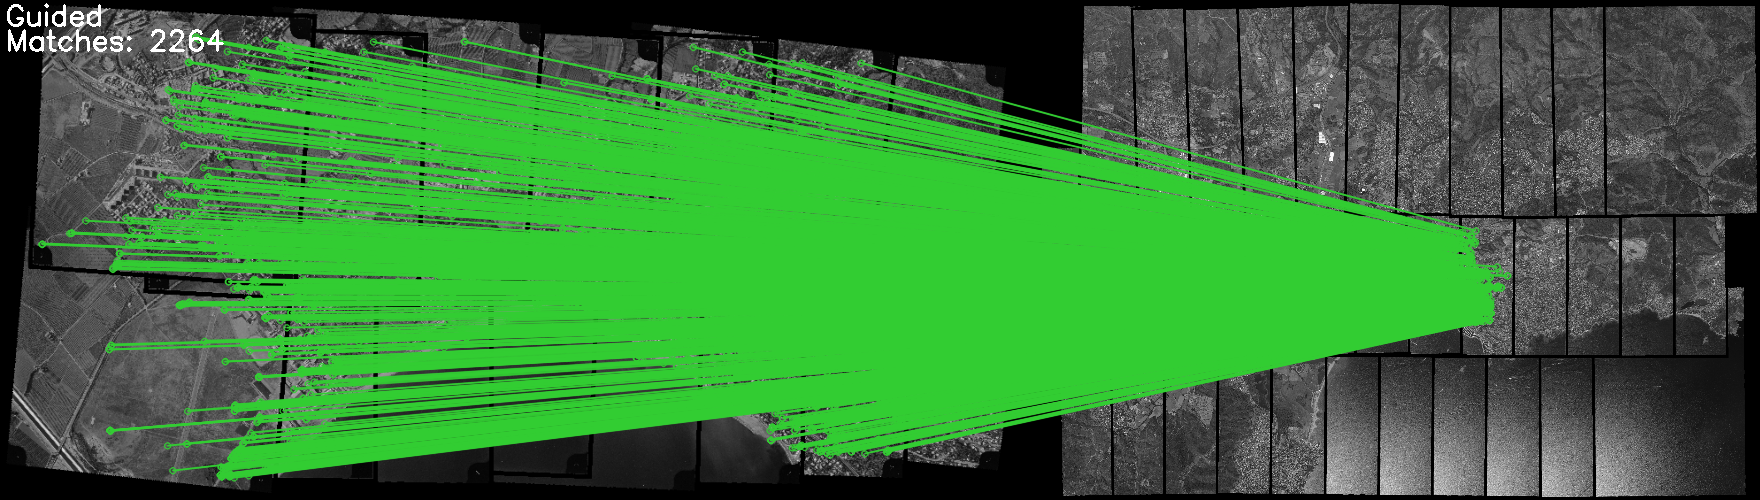
\includegraphics[width=6.8cm]{images/Chapitre4/Precise-SIFTDSMHomol-1966-2014-GuidedSIFT-3DRANSAC-CrossCorrelation-PileImg_Ortho-MEC-Malt_Tapas_1966_Ortho-MEC-Malt_2014.png}
			\end{minipage}%
		}
		\caption{Precise matching visualization of \textbf{Fr{\'e}jus 1966 and 2014}. (a) Image pairs to be matched, with red rectangles indicating the common zone. (b) Numbers of tentative, enhanced and final matches recovered with $Patch_{SpGDSM}$, $Guided_{SpGDSM}$, $Patch_{SIFTDSM}$ and $Guided_{SIFTDSM}$ individually. (c-f) Visualization of final matches recovered with $Patch_{SpGDSM}$, $Guided_{SpGDSM}$, $Patch_{SIFTDSM}$ and $Guided_{SIFTDSM}$ individually.}
		\label{MatchVizFrejus1966-2014}
	\end{center}
\end{figure*} 


\begin{figure*}[htbp]
	\begin{center}
		\subfigure[Common zone]{
			\begin{minipage}[t]{0.48\linewidth}
				\centering
				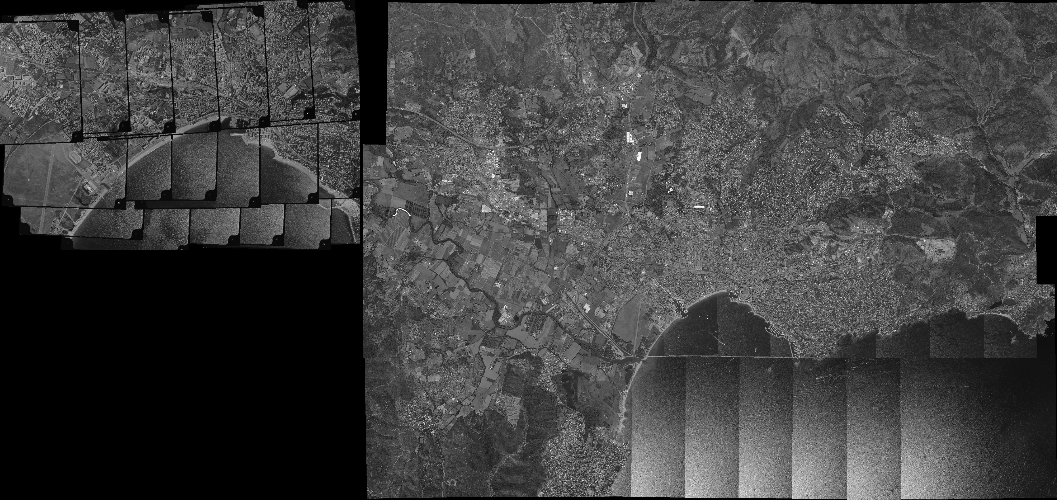
\includegraphics[width=6.8cm]{images/Chapitre3/Pseudo-Ortho-MEC-Malt_Tapas_1970_Ortho-MEC-Malt_2014.png}
			\end{minipage}%
		}
		\subfigure[Number of recovered matches]{
			\begin{minipage}[t]{0.48\linewidth}
				\centering
				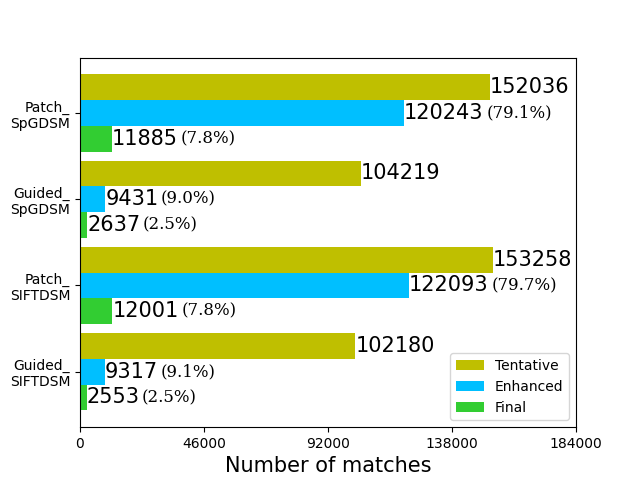
\includegraphics[width=5.8cm]{images/Chapitre4/PlotBarH-Frejus1970-2014.png}
			\end{minipage}%
		}
		\subfigure[$Patch_{SpGDSM}$]{
			\begin{minipage}[t]{0.48\linewidth}
				\centering
				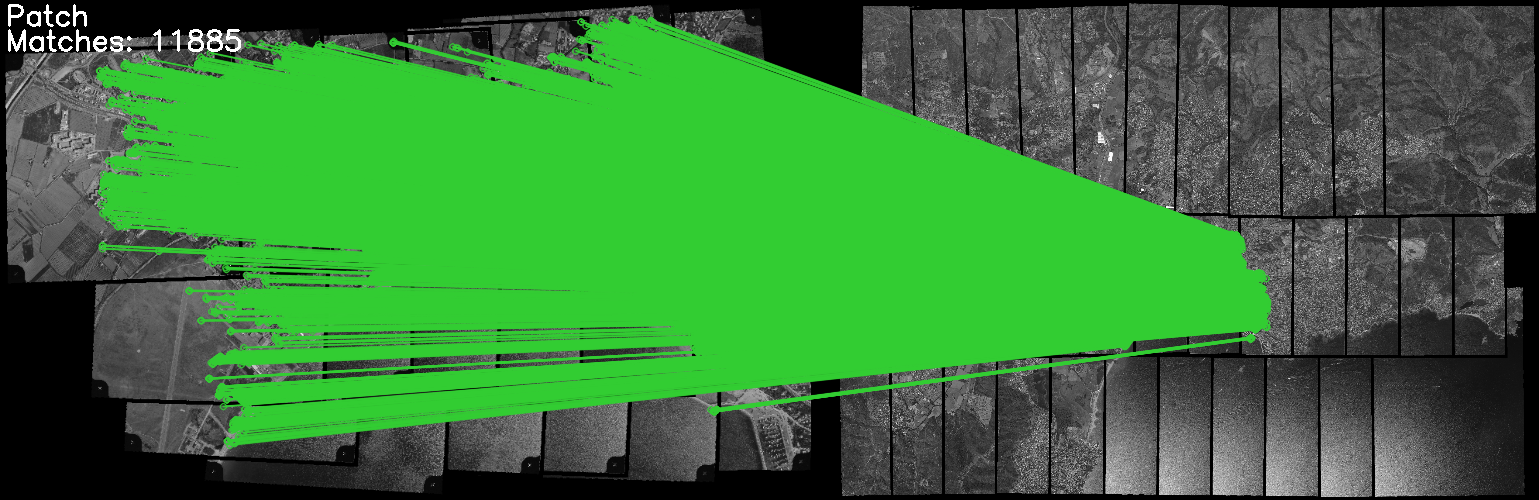
\includegraphics[width=6.8cm]{images/Chapitre4/Precise-SpGDSMHomol-1970-2014-SuperGlue-3DRANSAC-CrossCorrelation-PileImg_Ortho-MEC-Malt_Tapas_1970_Ortho-MEC-Malt_2014.png}
			\end{minipage}%
		}
		\subfigure[$Guided_{SpGDSM}$]{
			\begin{minipage}[t]{0.48\linewidth}
				\centering
				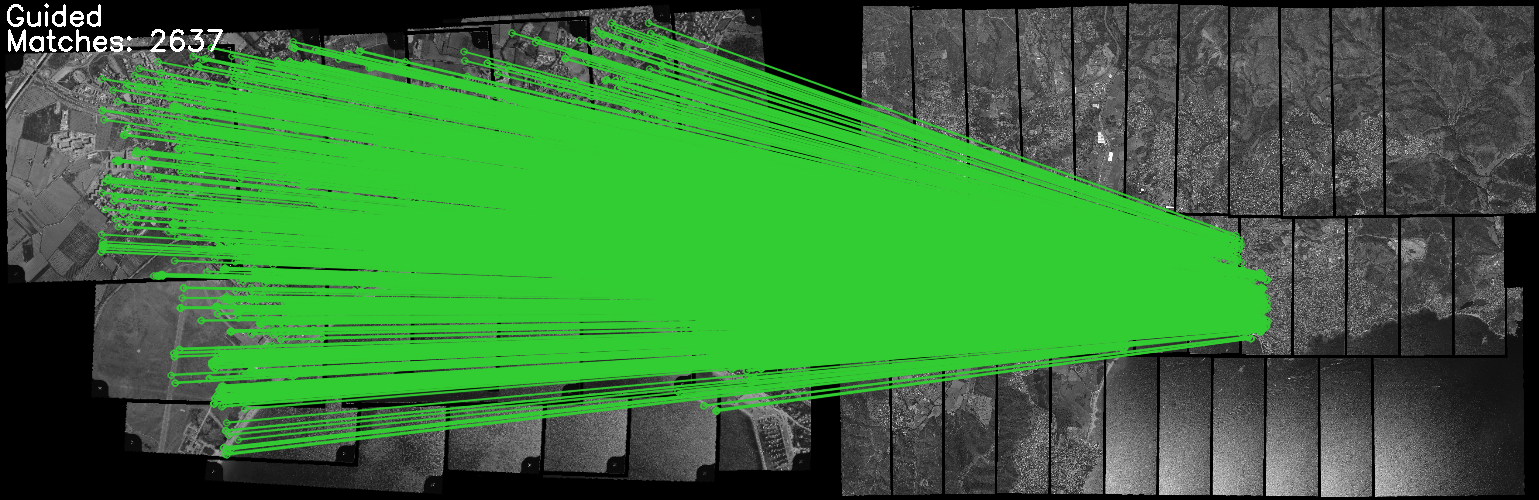
\includegraphics[width=6.8cm]{images/Chapitre4/Precise-SpGDSMHomol-1970-2014-GuidedSIFT-3DRANSAC-CrossCorrelation-PileImg_Ortho-MEC-Malt_Tapas_1970_Ortho-MEC-Malt_2014.png}
			\end{minipage}%
		}
		\subfigure[$Patch_{SIFTDSM}$]{
			\begin{minipage}[t]{0.48\linewidth}
				\centering
				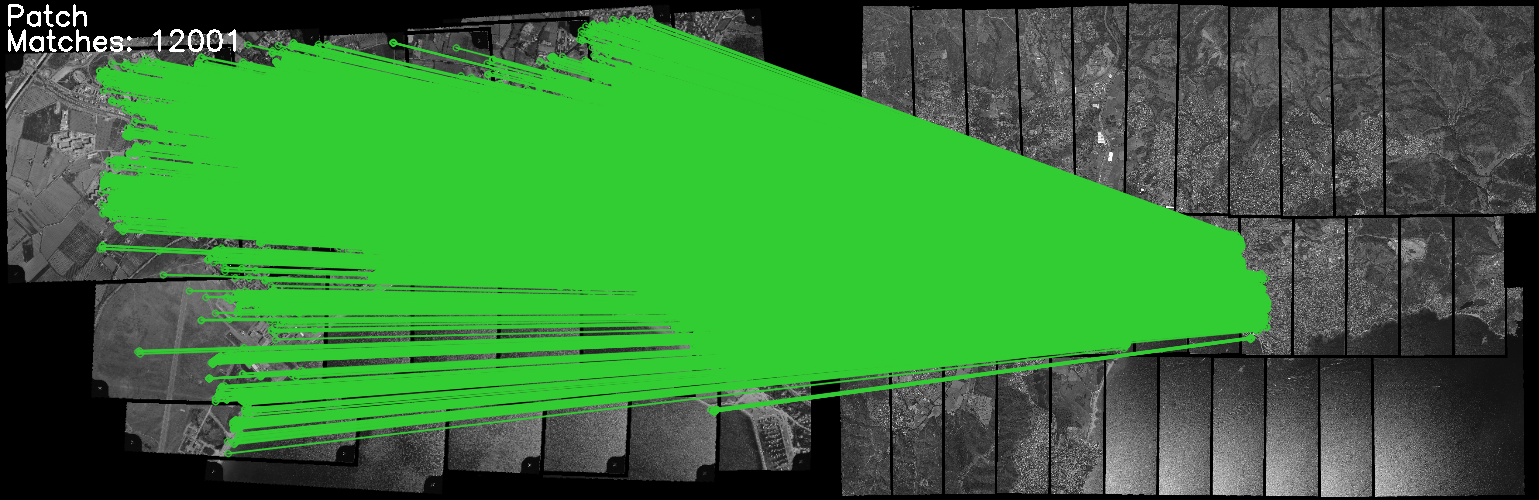
\includegraphics[width=6.8cm]{images/Chapitre4/Precise-SIFTDSMHomol-1970-2014-SuperGlue-3DRANSAC-CrossCorrelation-PileImg_Ortho-MEC-Malt_Tapas_1970_Ortho-MEC-Malt_2014.png}
			\end{minipage}%
		}
		\subfigure[$Guided_{SIFTDSM}$]{
			\begin{minipage}[t]{0.48\linewidth}
				\centering
				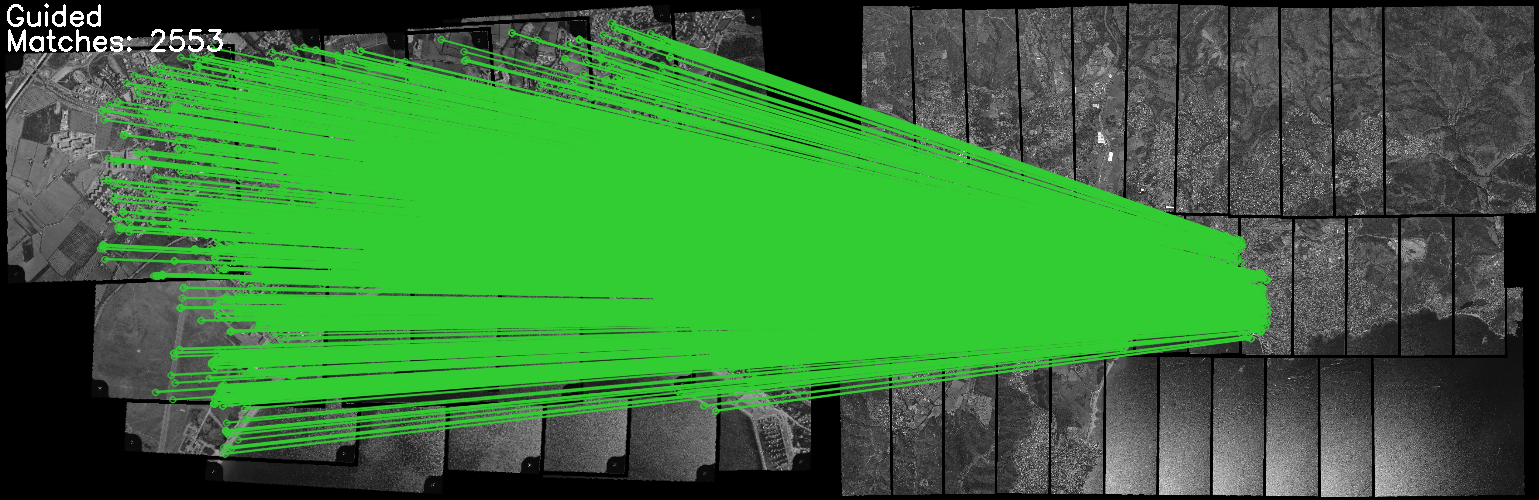
\includegraphics[width=6.8cm]{images/Chapitre4/Precise-SIFTDSMHomol-1970-2014-GuidedSIFT-3DRANSAC-CrossCorrelation-PileImg_Ortho-MEC-Malt_Tapas_1970_Ortho-MEC-Malt_2014.png}
			\end{minipage}%
		}
		\caption{Precise matching visualization of \textbf{Fr{\'e}jus 1970 and 2014}. (a) Image pairs to be matched, with red rectangles indicating the common zone. (b) Numbers of tentative, enhanced and final matches recovered with $Patch_{SpGDSM}$, $Guided_{SpGDSM}$, $Patch_{SIFTDSM}$ and $Guided_{SIFTDSM}$ individually. (c-f) Visualization of final matches recovered with $Patch_{SpGDSM}$, $Guided_{SpGDSM}$, $Patch_{SIFTDSM}$ and $Guided_{SIFTDSM}$ individually.}
		\label{MatchVizFrejus1970-2014}
	\end{center}
\end{figure*} 

%%%%%%%%%%%%%%%%%%Frejus histo

\begin{figure*}[htbp]
	\begin{center}
		\subfigure[Common zone]{
			\begin{minipage}[t]{0.48\linewidth}
				\centering
				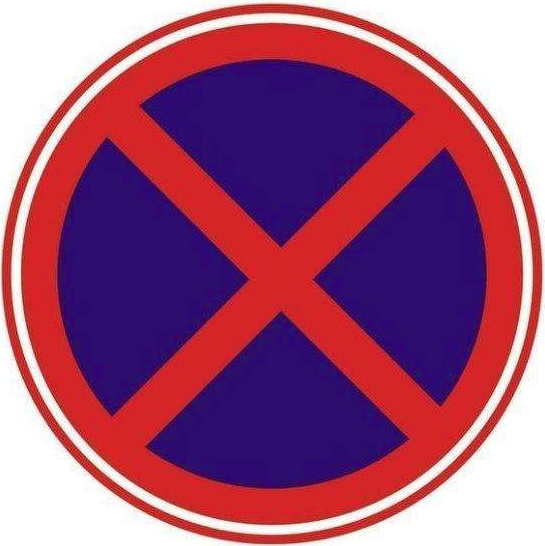
\includegraphics[width=6.8cm]{images/Chapitre4/Pseudo-Ortho-MEC-Malt_Tapas_1954_Ortho-MEC-Malt_Tapas_1970.png}
			\end{minipage}%
		}
		\subfigure[Number of recovered matches]{
			\begin{minipage}[t]{0.48\linewidth}
				\centering
				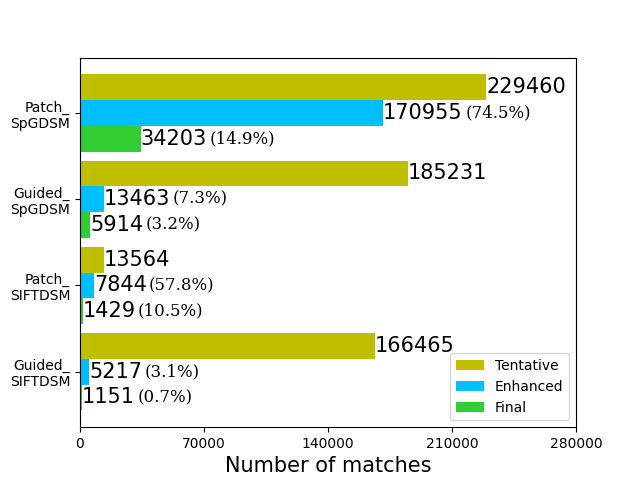
\includegraphics[width=5.8cm]{images/Chapitre4/PlotBarH-Frejus1954-1970.png}
			\end{minipage}%
		}
		\subfigure[$Patch_{SpGDSM}$]{
			\begin{minipage}[t]{0.48\linewidth}
				\centering
				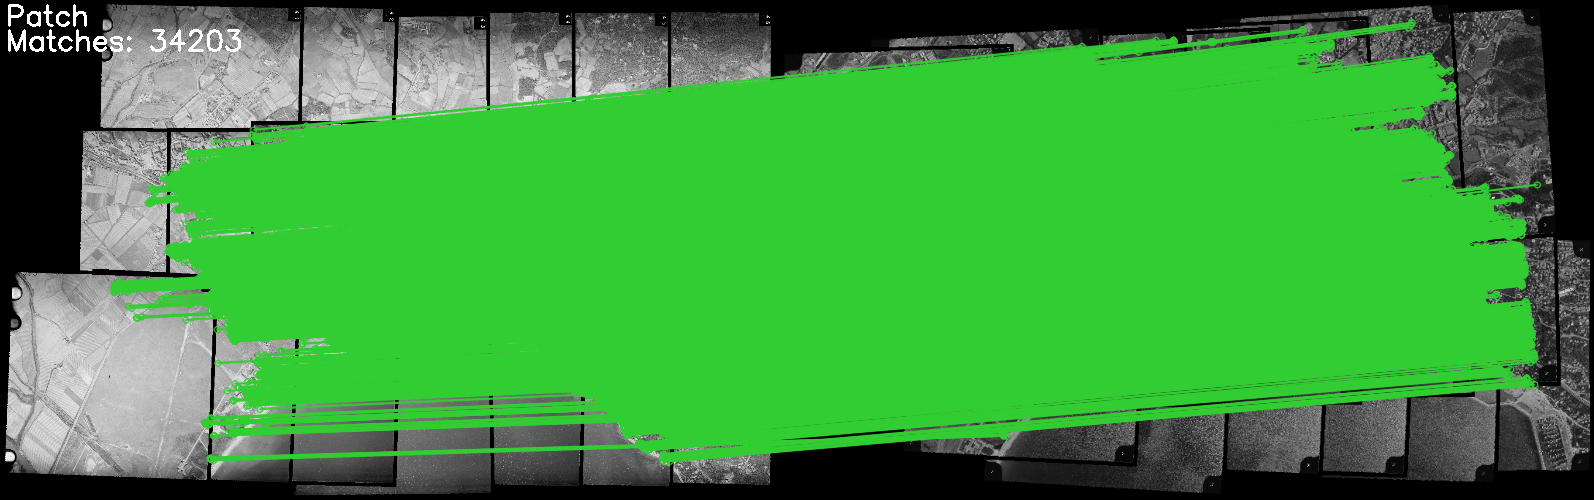
\includegraphics[width=6.8cm]{images/Chapitre4/Precise-SpGDSMHomol-1954-1970-SuperGlue-3DRANSAC-CrossCorrelation-PileImg_Ortho-MEC-Malt_Tapas_1954_Ortho-MEC-Malt_Tapas_1970.png}
			\end{minipage}%
		}
		\subfigure[$Guided_{SpGDSM}$]{
			\begin{minipage}[t]{0.48\linewidth}
				\centering
				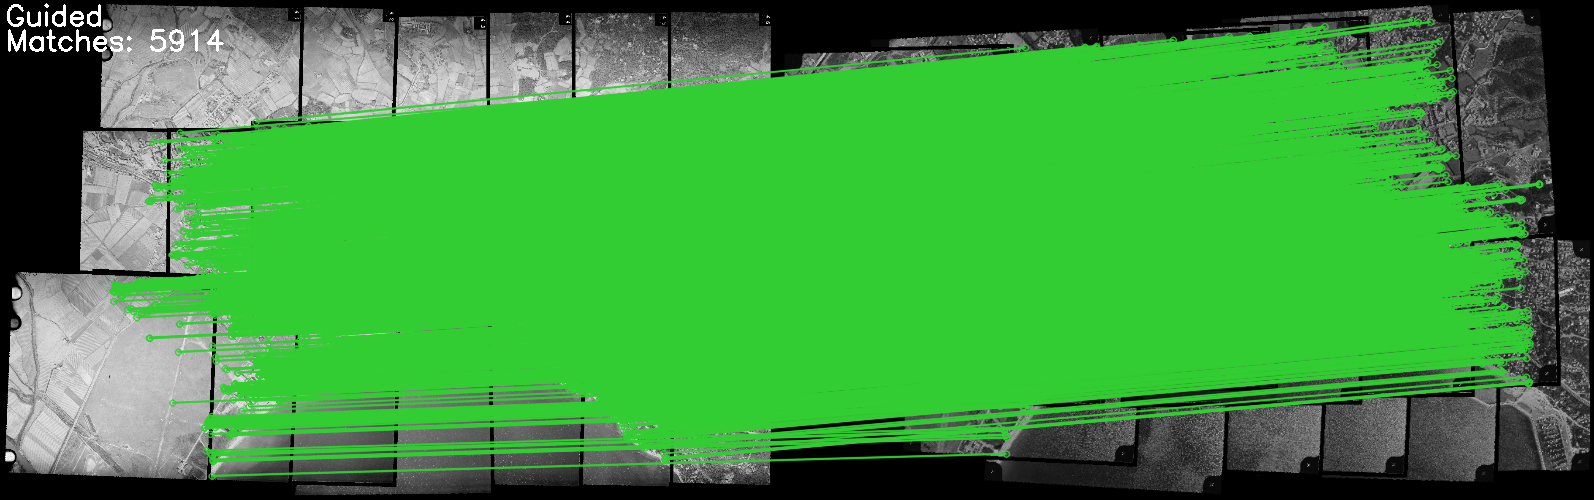
\includegraphics[width=6.8cm]{images/Chapitre4/Precise-SpGDSMHomol-1954-1970-GuidedSIFT-3DRANSAC-CrossCorrelation-PileImg_Ortho-MEC-Malt_Tapas_1954_Ortho-MEC-Malt_Tapas_1970.png}
			\end{minipage}%
		}
		\subfigure[$Patch_{SIFTDSM}$]{
			\begin{minipage}[t]{0.48\linewidth}
				\centering
				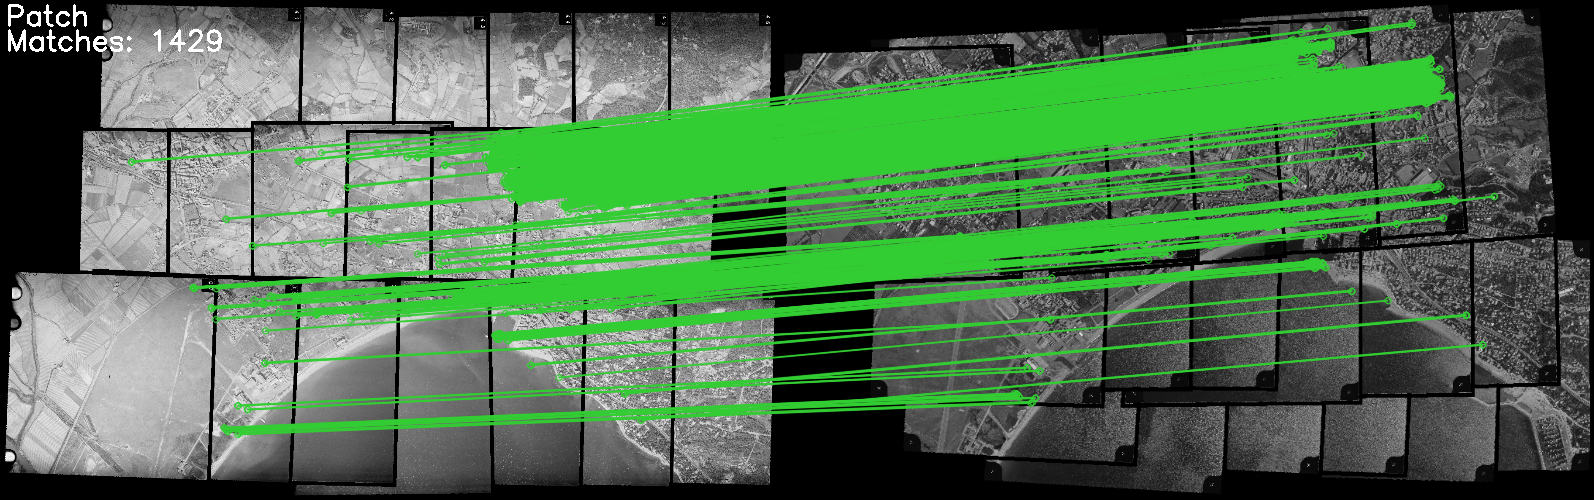
\includegraphics[width=6.8cm]{images/Chapitre4/Precise-SIFTDSMHomol-1954-1970-SuperGlue-3DRANSAC-CrossCorrelation-PileImg_Ortho-MEC-Malt_Tapas_1954_Ortho-MEC-Malt_Tapas_1970.png}
			\end{minipage}%
		}
		\subfigure[$Guided_{SIFTDSM}$]{
			\begin{minipage}[t]{0.48\linewidth}
				\centering
				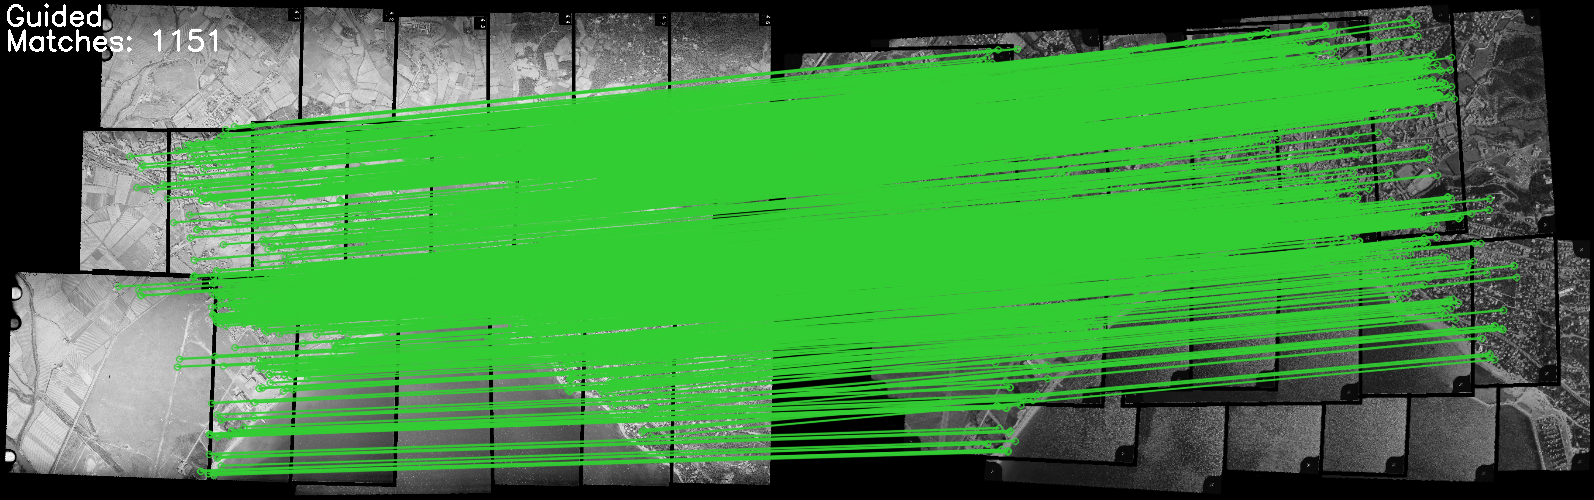
\includegraphics[width=6.8cm]{images/Chapitre4/Precise-SIFTDSMHomol-1954-1970-GuidedSIFT-3DRANSAC-CrossCorrelation-PileImg_Ortho-MEC-Malt_Tapas_1954_Ortho-MEC-Malt_Tapas_1970.png}
			\end{minipage}%
		}
		\caption{Precise matching visualization of \textbf{Fr{\'e}jus 1954 and 1970}. (a) Image pairs to be matched, with red rectangles indicating the common zone. (b) Numbers of tentative, enhanced and final matches recovered with $Patch_{SpGDSM}$, $Guided_{SpGDSM}$, $Patch_{SIFTDSM}$ and $Guided_{SIFTDSM}$ individually. (c-f) Visualization of final matches recovered with $Patch_{SpGDSM}$, $Guided_{SpGDSM}$, $Patch_{SIFTDSM}$ and $Guided_{SIFTDSM}$ individually.}
		\label{MatchVizFrejus1954-1970}
	\end{center}
\end{figure*} 



\begin{figure*}[htbp]
	\begin{center}
		\subfigure[Common zone]{
			\begin{minipage}[t]{0.48\linewidth}
				\centering
				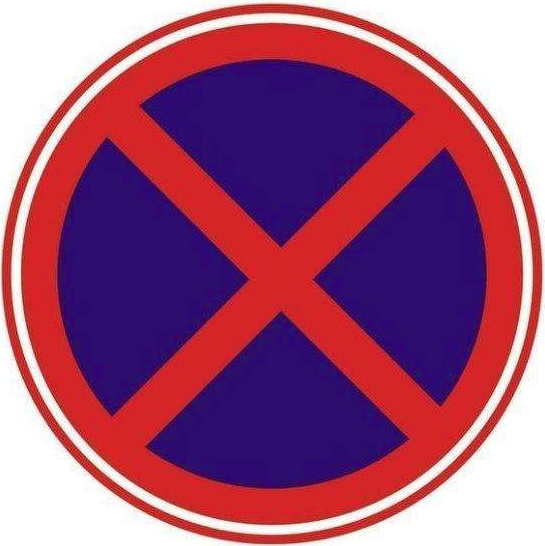
\includegraphics[width=6.8cm]{images/Chapitre4/Pseudo-Ortho-MEC-Malt_Tapas_1966_Ortho-MEC-Malt_Tapas_1970.png}
			\end{minipage}%
		}
		\subfigure[Number of recovered matches]{
			\begin{minipage}[t]{0.48\linewidth}
				\centering
				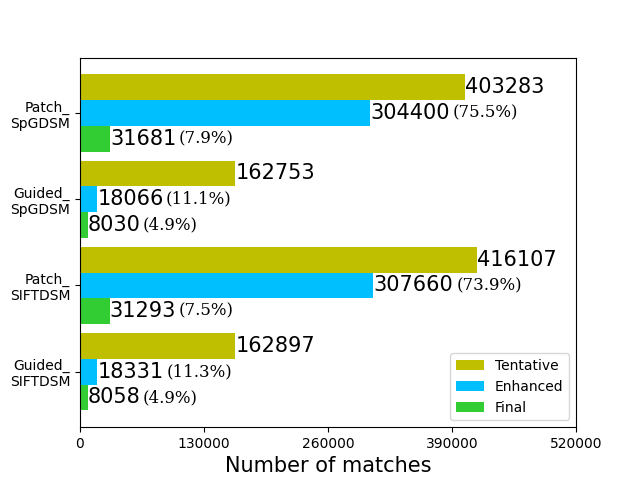
\includegraphics[width=5.8cm]{images/Chapitre4/PlotBarH-Frejus1966-1970.png}
			\end{minipage}%
		}
		\subfigure[$Patch_{SpGDSM}$]{
			\begin{minipage}[t]{0.48\linewidth}
				\centering
				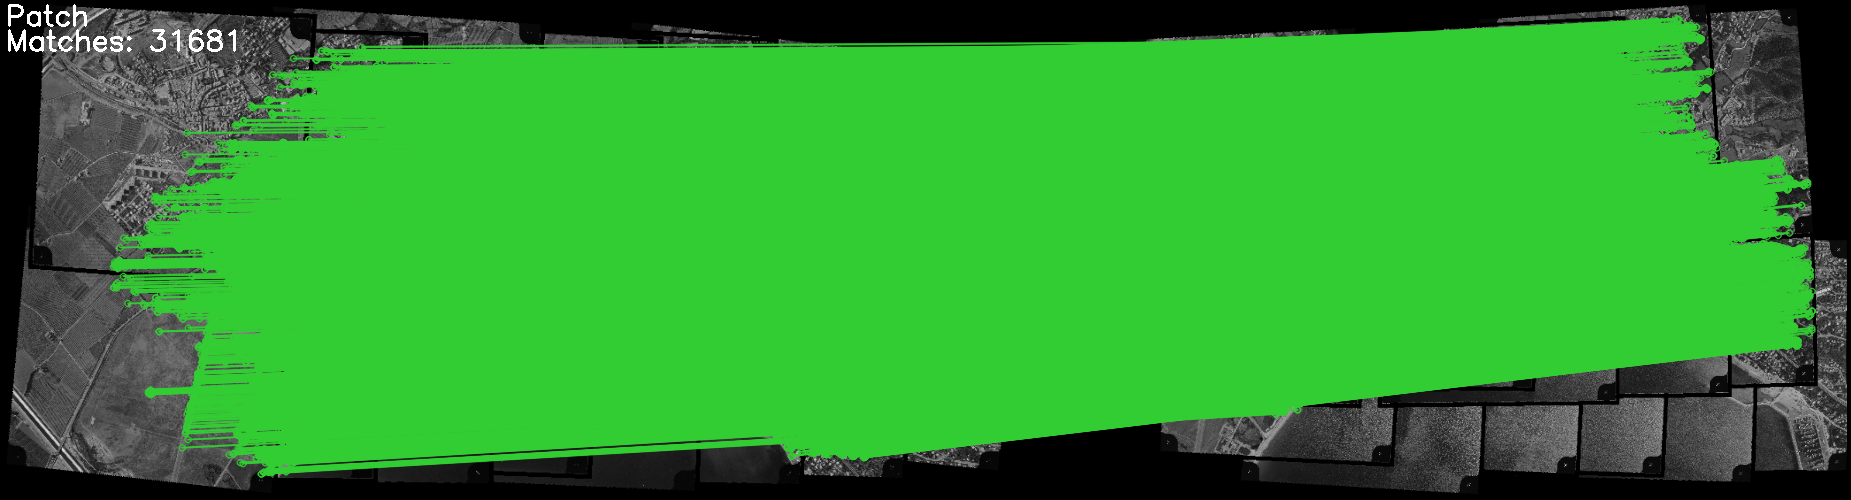
\includegraphics[width=6.8cm]{images/Chapitre4/Precise-SpGDSMHomol-1966-1970-SuperGlue-3DRANSAC-CrossCorrelation-PileImg_Ortho-MEC-Malt_Tapas_1966_Ortho-MEC-Malt_Tapas_1970.png}
			\end{minipage}%
		}
		\subfigure[$Guided_{SpGDSM}$]{
			\begin{minipage}[t]{0.48\linewidth}
				\centering
				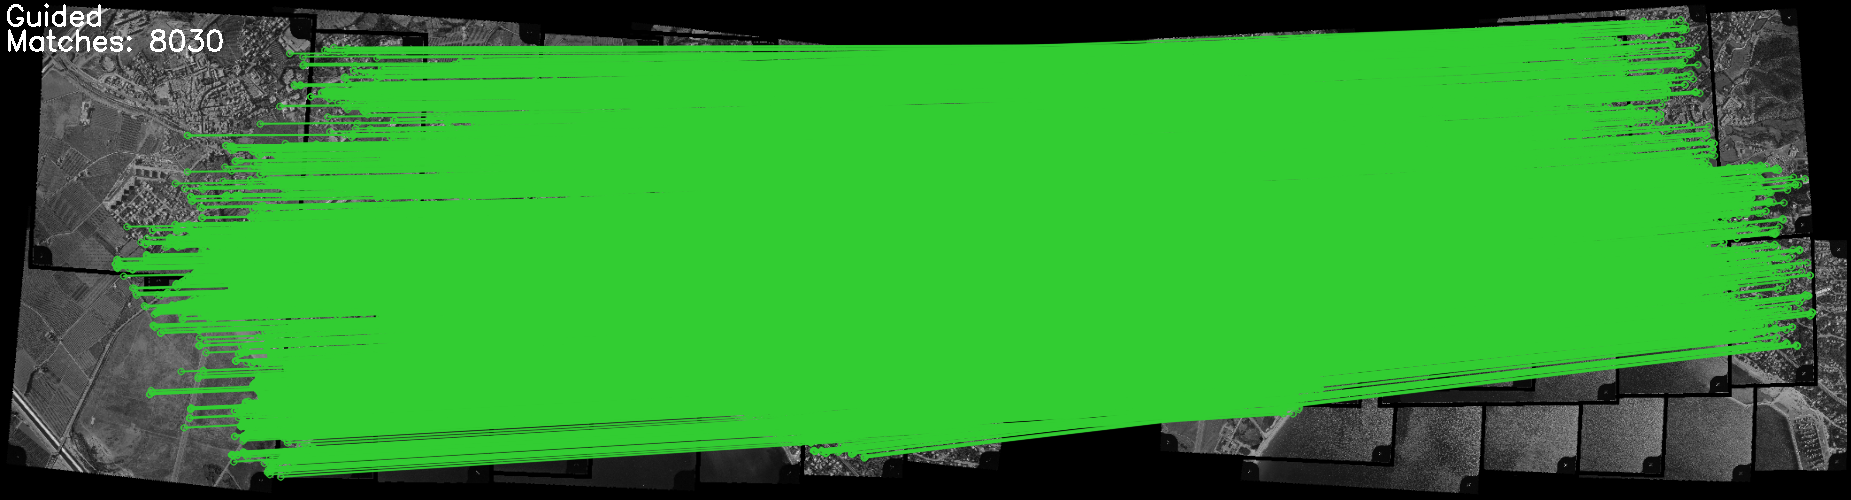
\includegraphics[width=6.8cm]{images/Chapitre4/Precise-SpGDSMHomol-1966-1970-GuidedSIFT-3DRANSAC-CrossCorrelation-PileImg_Ortho-MEC-Malt_Tapas_1966_Ortho-MEC-Malt_Tapas_1970.png}
			\end{minipage}%
		}
		\subfigure[$Patch_{SIFTDSM}$]{
			\begin{minipage}[t]{0.48\linewidth}
				\centering
				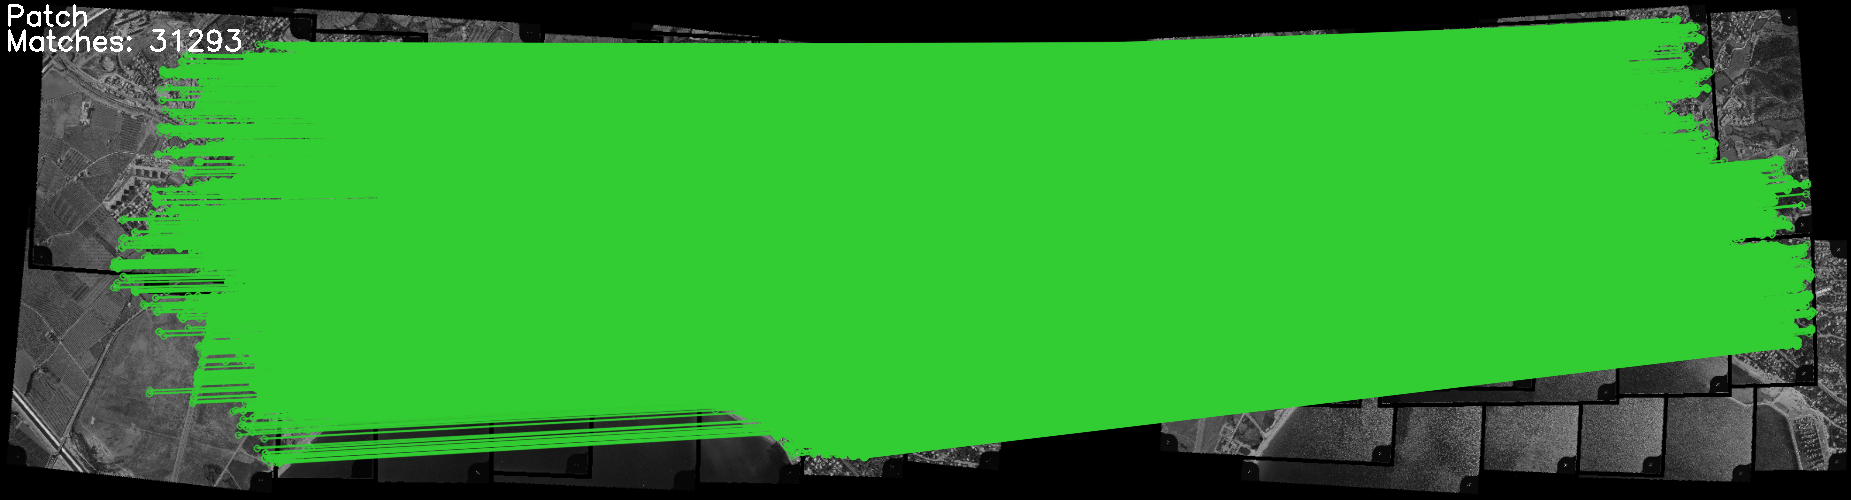
\includegraphics[width=6.8cm]{images/Chapitre4/Precise-SIFTDSMHomol-1966-1970-SuperGlue-3DRANSAC-CrossCorrelation-PileImg_Ortho-MEC-Malt_Tapas_1966_Ortho-MEC-Malt_Tapas_1970.png}
			\end{minipage}%
		}
		\subfigure[$Guided_{SIFTDSM}$]{
			\begin{minipage}[t]{0.48\linewidth}
				\centering
				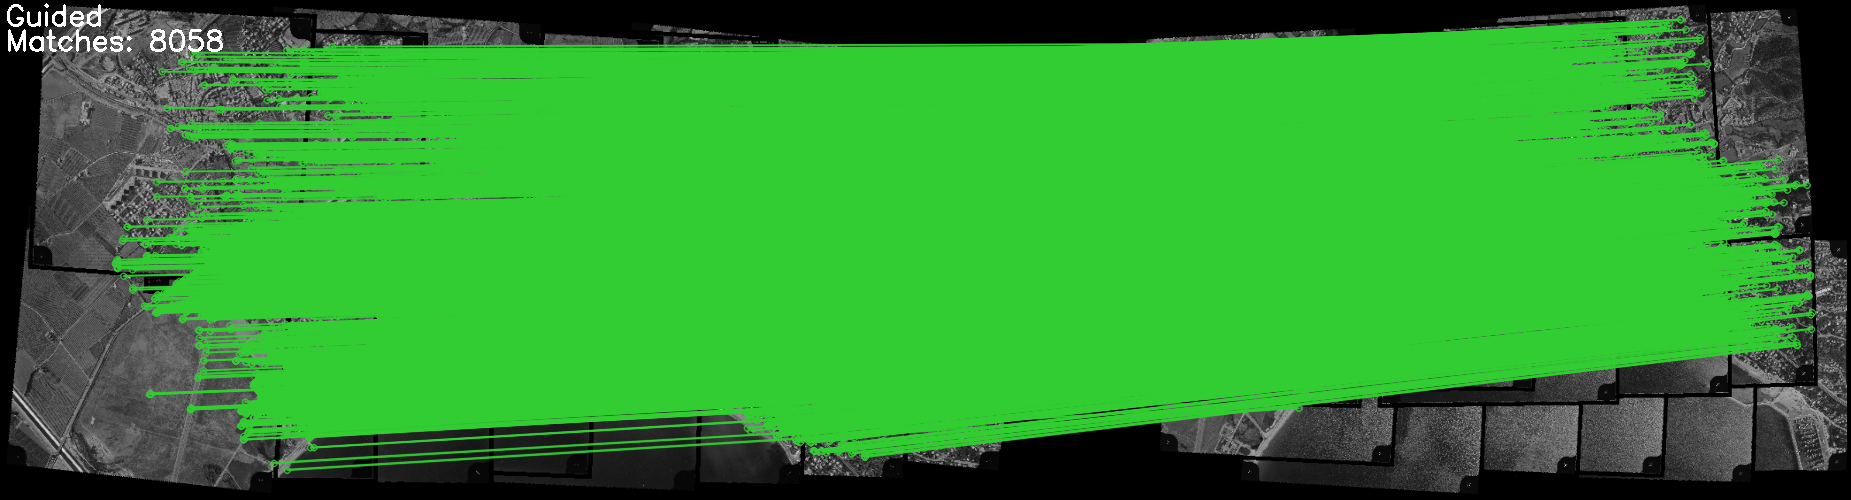
\includegraphics[width=6.8cm]{images/Chapitre4/Precise-SIFTDSMHomol-1966-1970-GuidedSIFT-3DRANSAC-CrossCorrelation-PileImg_Ortho-MEC-Malt_Tapas_1966_Ortho-MEC-Malt_Tapas_1970.png}
			\end{minipage}%
		}
		\caption{Precise matching visualization of \textbf{Fr{\'e}jus 1966 and 1970}. (a) Image pairs to be matched, with red rectangles indicating the common zone. (b) Numbers of tentative, enhanced and final matches recovered with $Patch_{SpGDSM}$, $Guided_{SpGDSM}$, $Patch_{SIFTDSM}$ and $Guided_{SIFTDSM}$ individually. (c-f) Visualization of final matches recovered with $Patch_{SpGDSM}$, $Guided_{SpGDSM}$, $Patch_{SIFTDSM}$ and $Guided_{SIFTDSM}$ individually.}
		\label{MatchVizFrejus1966-1970}
	\end{center}
\end{figure*} 


\begin{figure*}[htbp]
	\begin{center}
		\subfigure[Common zone]{
			\begin{minipage}[t]{0.48\linewidth}
				\centering
				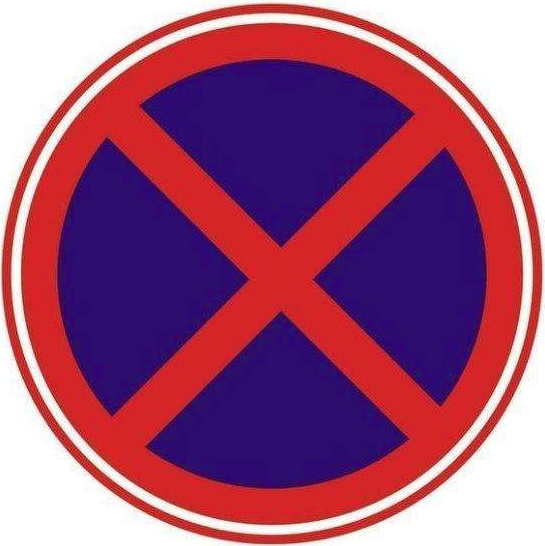
\includegraphics[width=6.8cm]{images/Chapitre4/Pseudo-Ortho-MEC-Malt_Tapas_1954_Ortho-MEC-Malt_Tapas_1966.png}
			\end{minipage}%
		}
		\subfigure[Number of recovered matches]{
			\begin{minipage}[t]{0.48\linewidth}
				\centering
				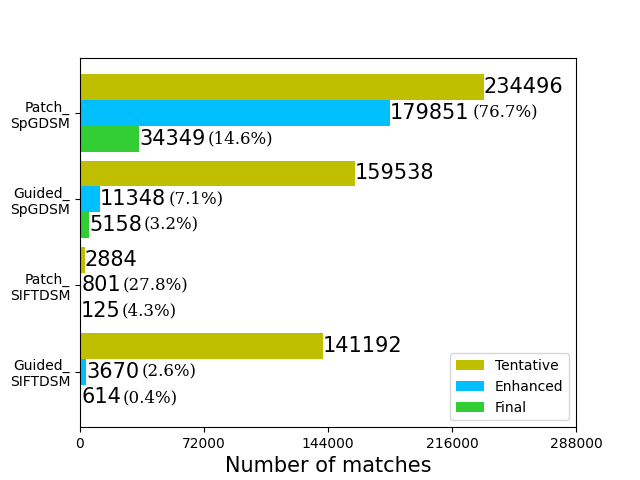
\includegraphics[width=5.8cm]{images/Chapitre4/PlotBarH-Frejus1954-1966.png}
			\end{minipage}%
		}
		\subfigure[$Patch_{SpGDSM}$]{
			\begin{minipage}[t]{0.48\linewidth}
				\centering
				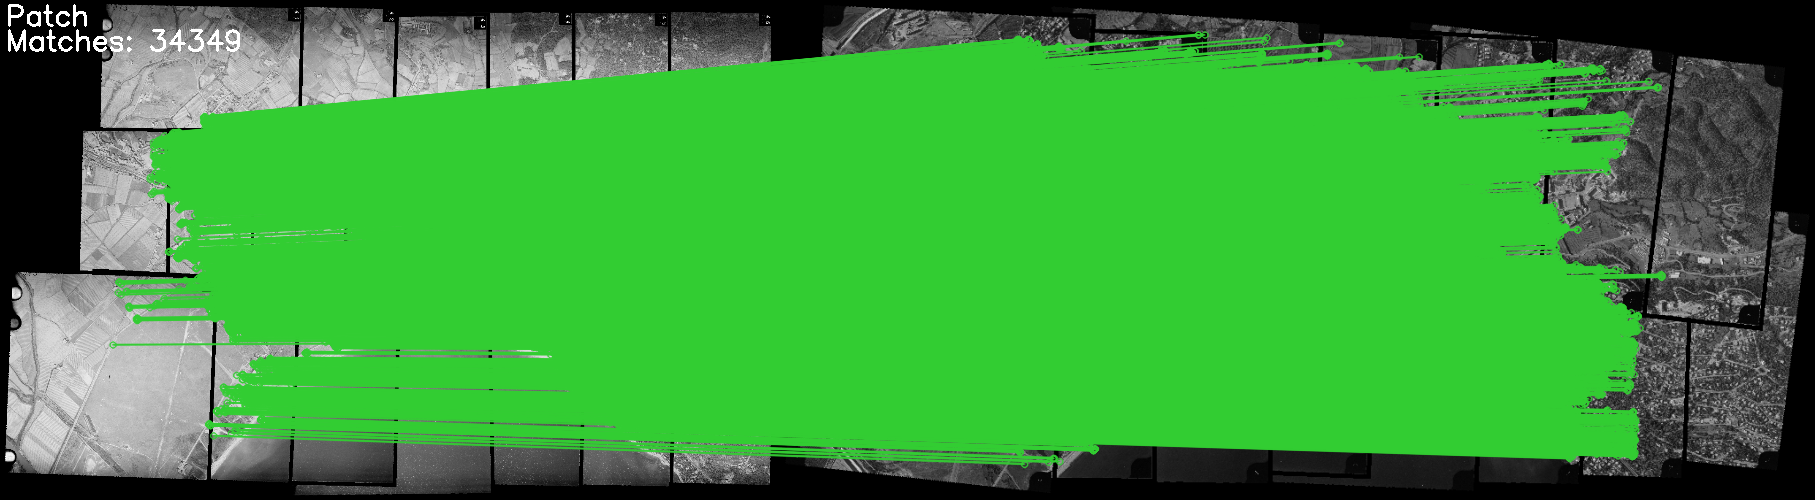
\includegraphics[width=6.8cm]{images/Chapitre4/Precise-SpGDSMHomol-1954-1966-SuperGlue-3DRANSAC-CrossCorrelation-PileImg_Ortho-MEC-Malt_Tapas_1954_Ortho-MEC-Malt_Tapas_1966.png}
			\end{minipage}%
		}
		\subfigure[$Guided_{SpGDSM}$]{
			\begin{minipage}[t]{0.48\linewidth}
				\centering
				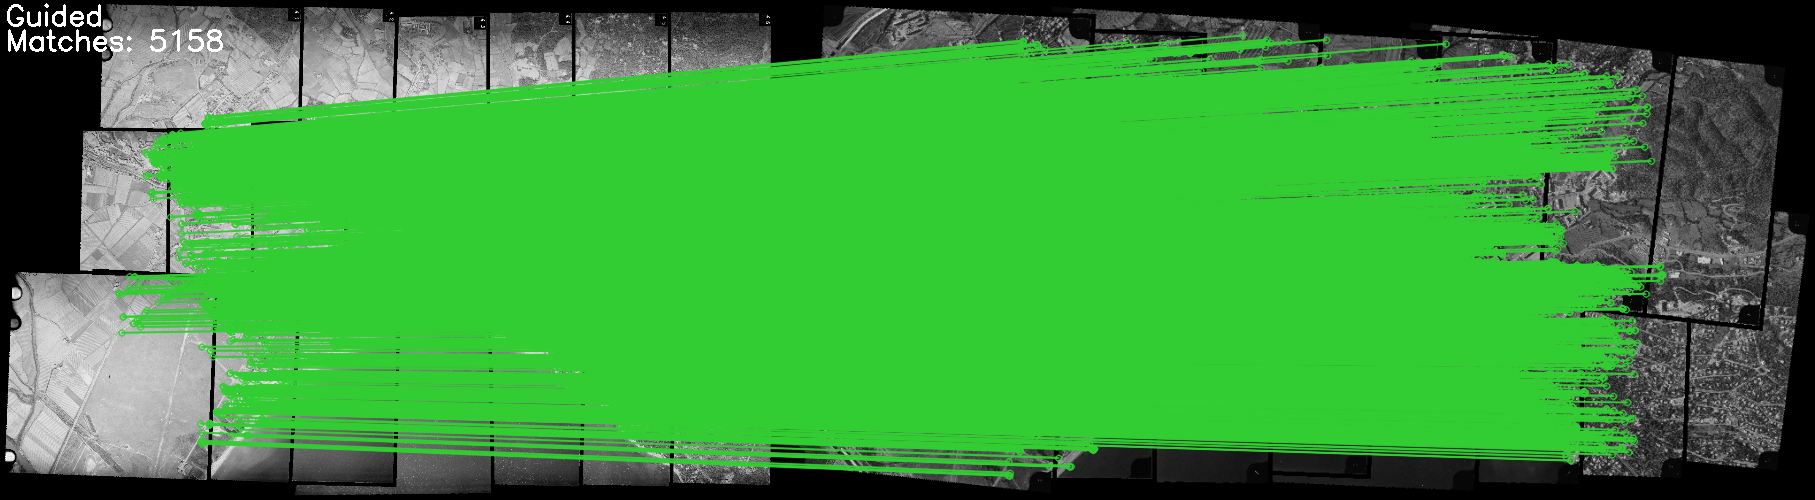
\includegraphics[width=6.8cm]{images/Chapitre4/Precise-SpGDSMHomol-1954-1966-GuidedSIFT-3DRANSAC-CrossCorrelation-PileImg_Ortho-MEC-Malt_Tapas_1954_Ortho-MEC-Malt_Tapas_1966.png}
			\end{minipage}%
		}
		\subfigure[$Patch_{SIFTDSM}$]{
			\begin{minipage}[t]{0.48\linewidth}
				\centering
				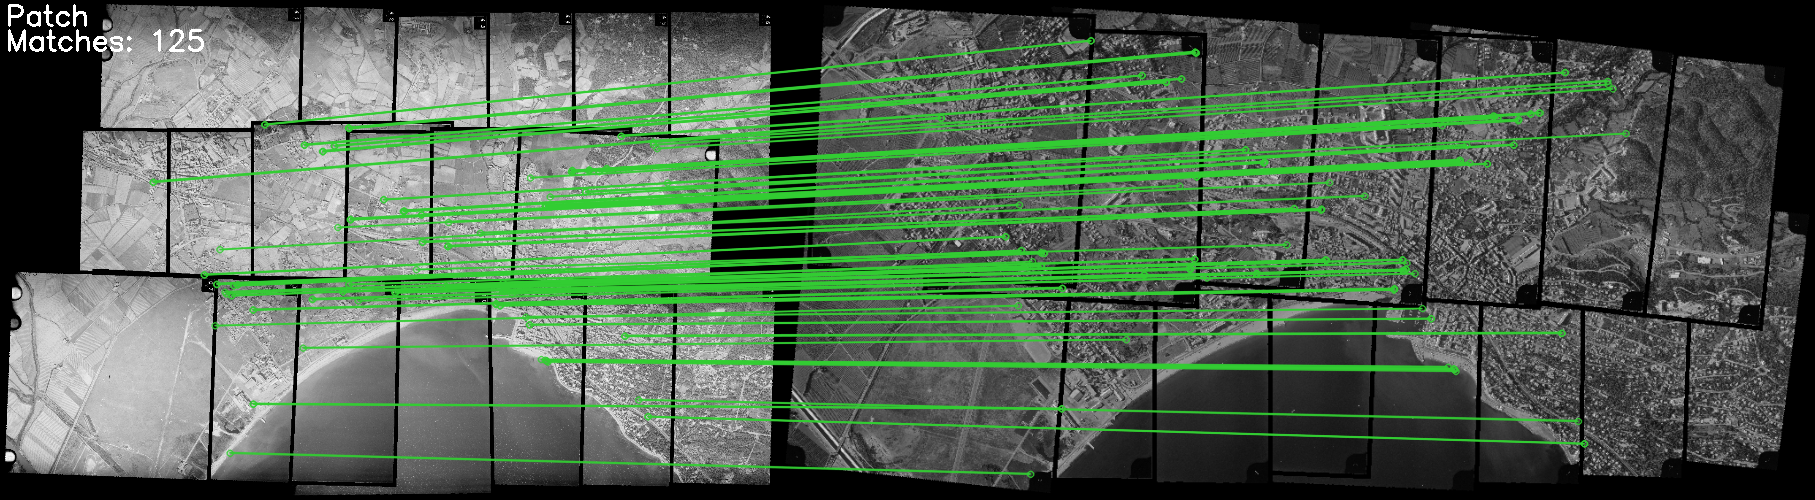
\includegraphics[width=6.8cm]{images/Chapitre4/Precise-SIFTDSMHomol-1954-1966-SuperGlue-3DRANSAC-CrossCorrelation-PileImg_Ortho-MEC-Malt_Tapas_1954_Ortho-MEC-Malt_Tapas_1966.png}
			\end{minipage}%
		}
		\subfigure[$Guided_{SIFTDSM}$]{
			\begin{minipage}[t]{0.48\linewidth}
				\centering
				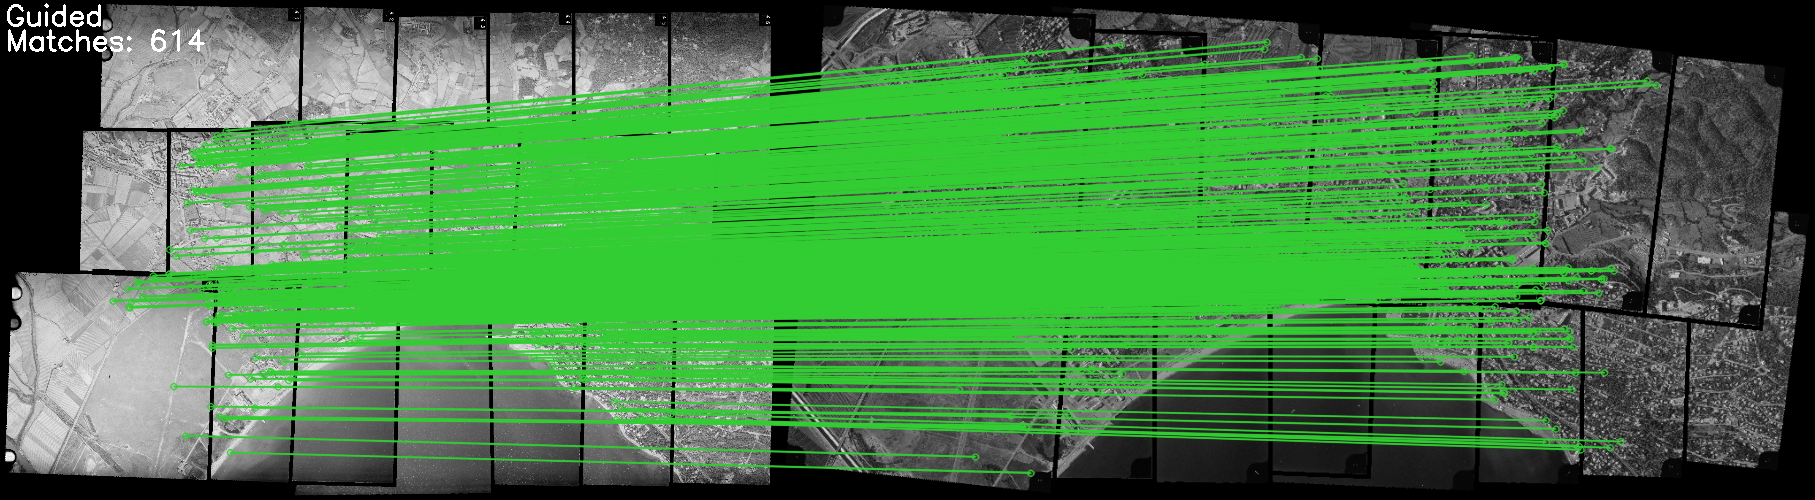
\includegraphics[width=6.8cm]{images/Chapitre4/Precise-SIFTDSMHomol-1954-1966-GuidedSIFT-3DRANSAC-CrossCorrelation-PileImg_Ortho-MEC-Malt_Tapas_1954_Ortho-MEC-Malt_Tapas_1966.png}
			\end{minipage}%
		}
		\caption{Precise matching visualization of \textbf{Fr{\'e}jus 1954 and 1966}. (a) Image pairs to be matched, with red rectangles indicating the common zone. (b) Numbers of tentative, enhanced and final matches recovered with $Patch_{SpGDSM}$, $Guided_{SpGDSM}$, $Patch_{SIFTDSM}$ and $Guided_{SIFTDSM}$ individually. (c-f) Visualization of final matches recovered with $Patch_{SpGDSM}$, $Guided_{SpGDSM}$, $Patch_{SIFTDSM}$ and $Guided_{SIFTDSM}$ individually.}
		\label{MatchVizFrejus1954-1966}
	\end{center}
\end{figure*} 

%%%%%%%%%%%%%%%%%Pezenas
\begin{figure*}[htbp]
	\begin{center}
		\subfigure[Common zone]{
			\begin{minipage}[t]{0.48\linewidth}
				\centering
				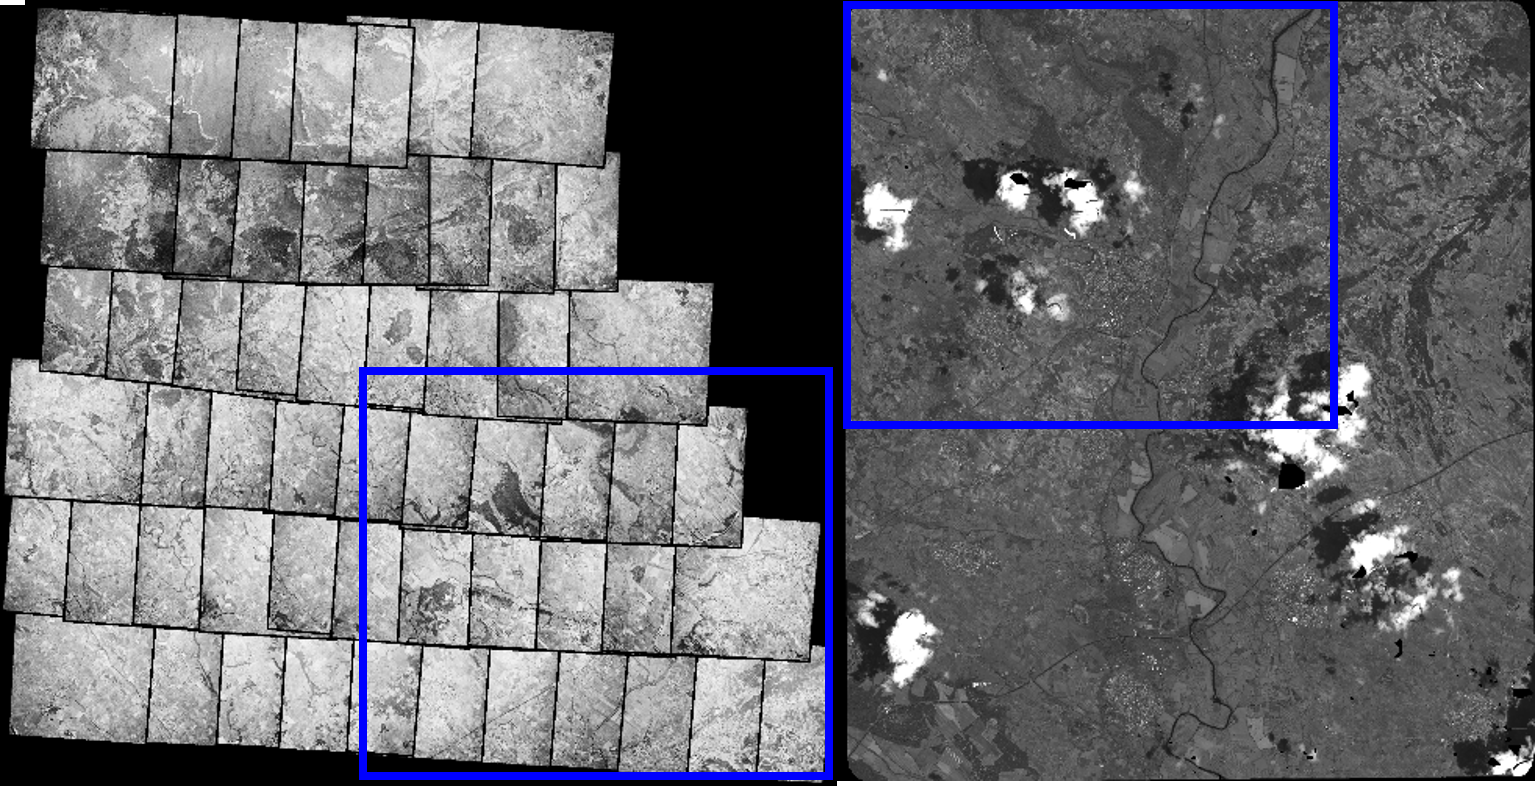
\includegraphics[width=6.8cm]{images/Chapitre4/Pseudo-Ortho-MEC-Malt_Tapas_1971_Ortho-MEC-Malt_Satellite.png}
			\end{minipage}%
		}
		\subfigure[Number of recovered matches]{
			\begin{minipage}[t]{0.48\linewidth}
				\centering
				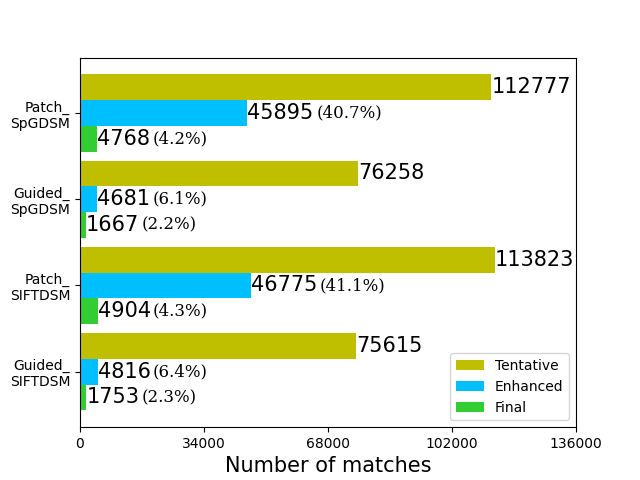
\includegraphics[width=5.8cm]{images/Chapitre4/PlotBarH-Pezenas1971-2014.png}
			\end{minipage}%
		}
		\subfigure[$Patch_{SpGDSM}$]{
			\begin{minipage}[t]{0.48\linewidth}
				\centering
				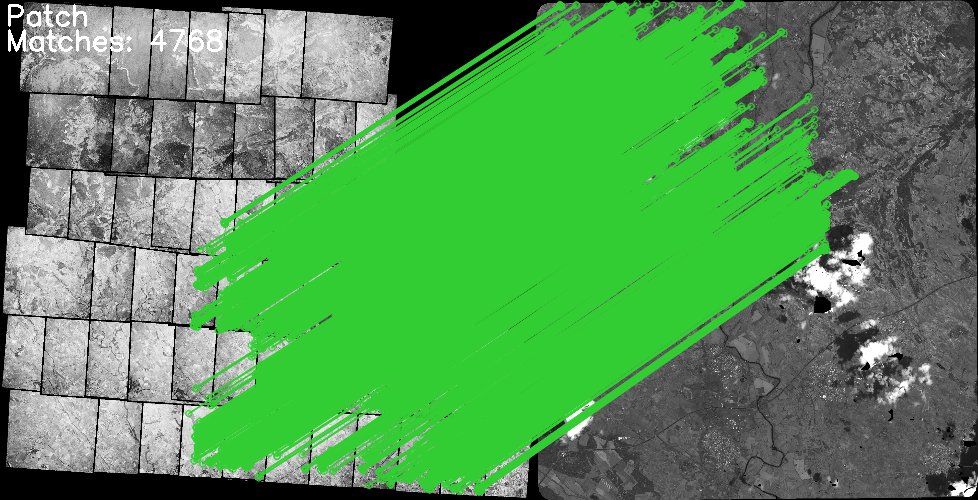
\includegraphics[width=6.8cm]{images/Chapitre4/Precise-SpGDSMHomol-SuperGlue-3DRANSAC-CrossCorrelation-PileImg_Ortho-MEC-Malt_Tapas_1971_Ortho-MEC-Malt_Satellite.png}
			\end{minipage}%
		}
		\subfigure[$Guided_{SpGDSM}$]{
			\begin{minipage}[t]{0.48\linewidth}
				\centering
				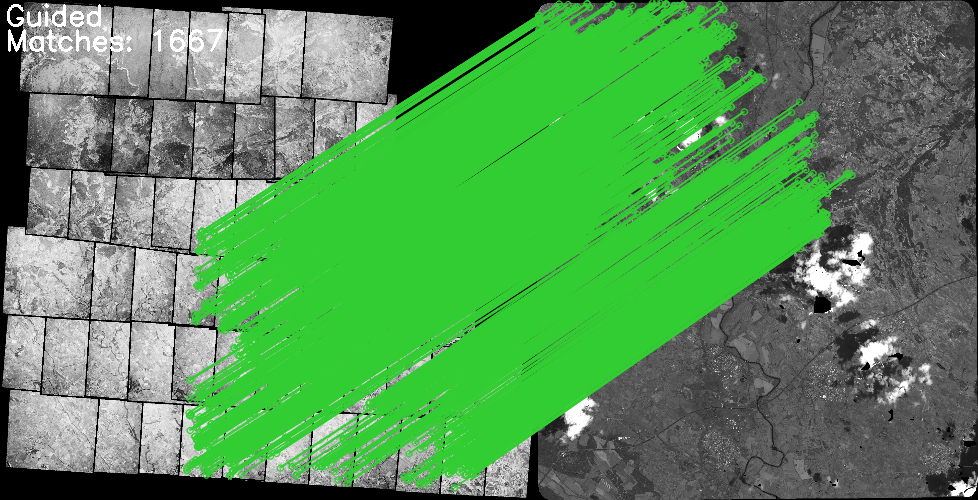
\includegraphics[width=6.8cm]{images/Chapitre4/Precise-SpGDSMHomol-GuidedSIFT-3DRANSAC-CrossCorrelation-PileImg_Ortho-MEC-Malt_Tapas_1971_Ortho-MEC-Malt_Satellite.png}
			\end{minipage}%
		}
		\subfigure[$Patch_{SIFTDSM}$]{
			\begin{minipage}[t]{0.48\linewidth}
				\centering
				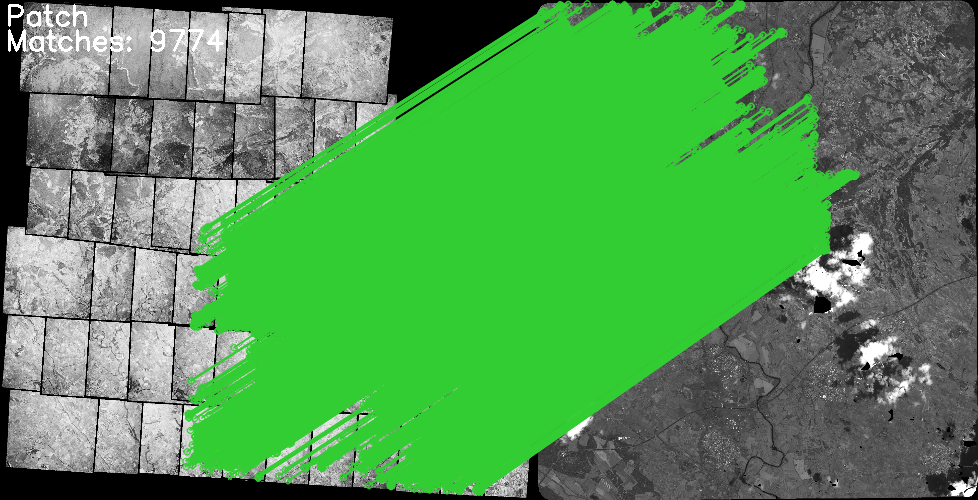
\includegraphics[width=6.8cm]{images/Chapitre4/Precise-SIFTDSMHomol-SuperGlue-3DRANSAC-CrossCorrelation-PileImg_Ortho-MEC-Malt_Tapas_1971_Ortho-MEC-Malt_Satellite.png}
			\end{minipage}%
		}
		\subfigure[$Guided_{SIFTDSM}$]{
			\begin{minipage}[t]{0.48\linewidth}
				\centering
				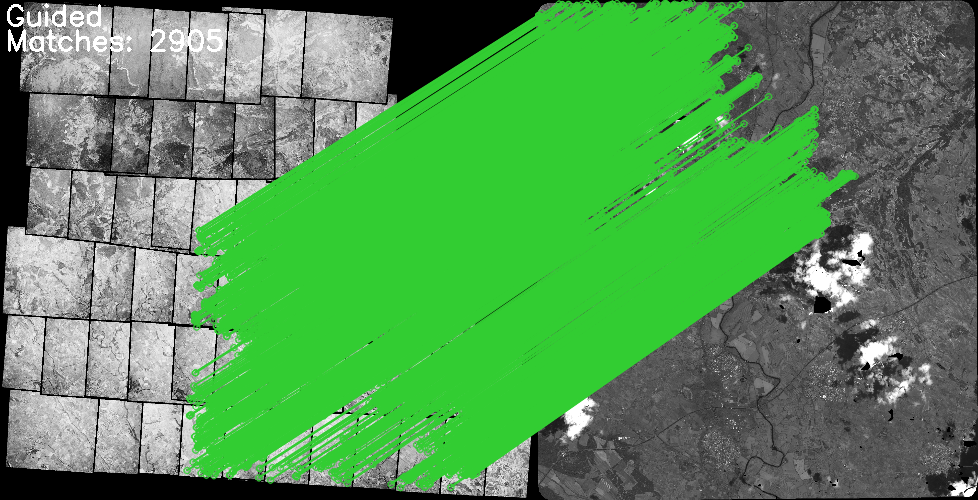
\includegraphics[width=6.8cm]{images/Chapitre4/Precise-SIFTDSMHomol-GuidedSIFT-3DRANSAC-CrossCorrelation-PileImg_Ortho-MEC-Malt_Tapas_1971_Ortho-MEC-Malt_Satellite.png}
			\end{minipage}%
		}
		\caption{Precise matching visualization of \textbf{Pezenas 1971 and 2014 (Satellite)}. (a) Image pairs to be matched, with red rectangles indicating the common zone. (b) Numbers of tentative, enhanced and final matches recovered with $Patch_{SpGDSM}$, $Guided_{SpGDSM}$, $Patch_{SIFTDSM}$ and $Guided_{SIFTDSM}$ individually. (c-f) Visualization of final matches recovered with $Patch_{SpGDSM}$, $Guided_{SpGDSM}$, $Patch_{SIFTDSM}$ and $Guided_{SIFTDSM}$ individually.}
		\label{MatchVizPezenas}
	\end{center}
\end{figure*} 

%Pseudo-Ortho-MEC-Malt_Tapas_1991_Ortho-MEC-Malt_Tapas_1994

\begin{figure*}[htbp]
	\begin{center}
		\subfigure[Common zone]{
			\begin{minipage}[t]{0.48\linewidth}
				\centering
				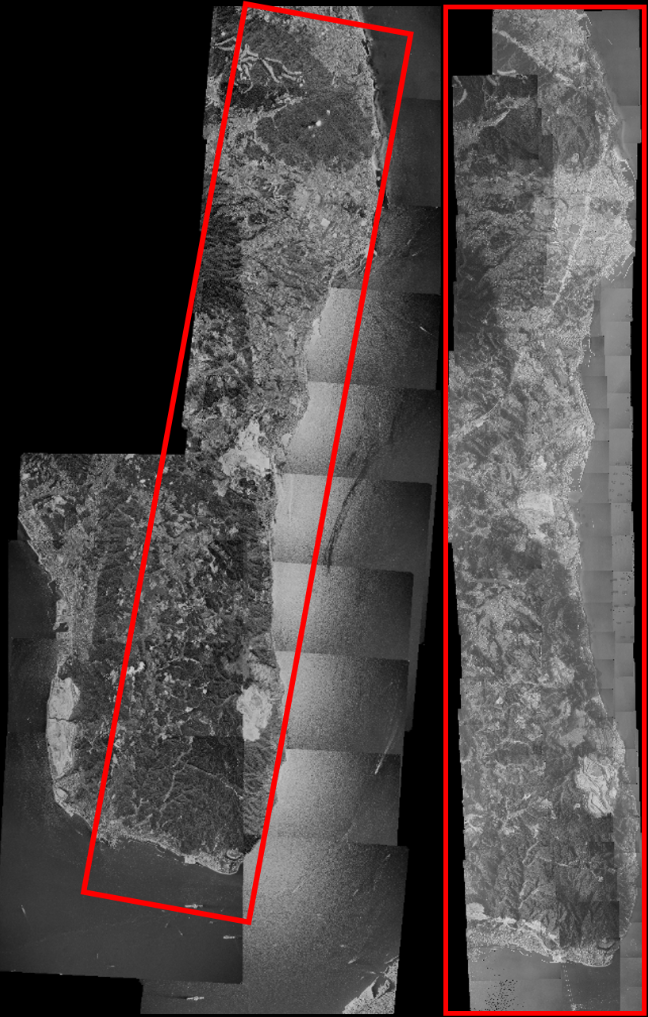
\includegraphics[width=3.8cm,angle=90]{images/Chapitre3/Pseudo-Ortho-MEC-Malt_Tapas_1991_Ortho-MEC-Malt_Tapas_1994.png}
			\end{minipage}%
		}
		\subfigure[Number of recovered matches]{
			\begin{minipage}[t]{0.48\linewidth}
				\centering
				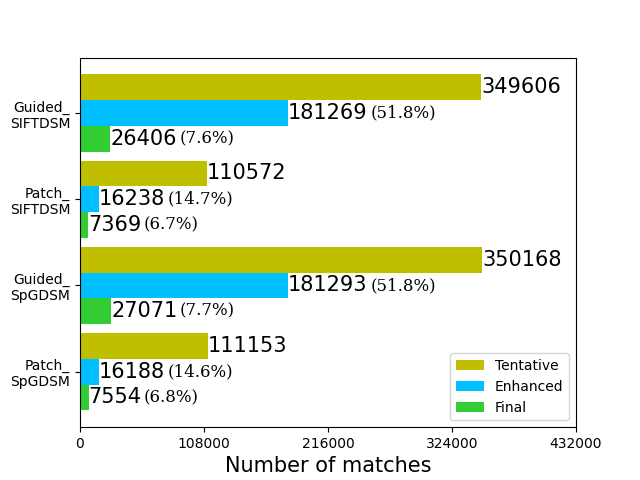
\includegraphics[width=5.8cm]{images/Chapitre4/PlotBarH-Kobe1991-1995.png}
			\end{minipage}%
		}
		\subfigure[$Patch_{SpGDSM}$]{
			\begin{minipage}[t]{0.48\linewidth}
				\centering
				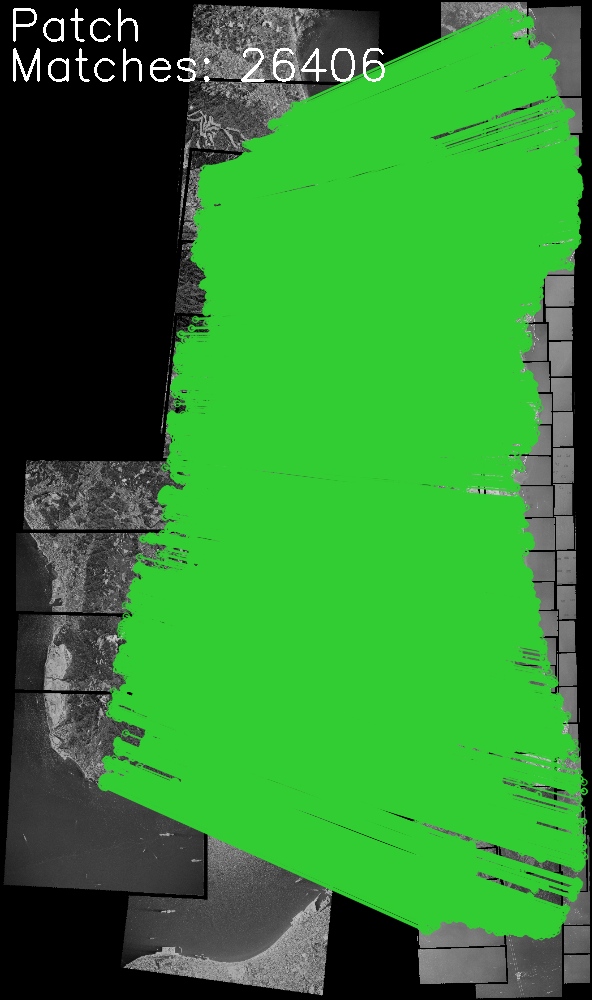
\includegraphics[width=3.8cm,angle=90]{images/Chapitre4/Precise-SpGDSMHomol-SuperGlue-3DRANSAC-CrossCorrelation-PileImg_Ortho-MEC-Malt_Tapas_1991_Ortho-MEC-Malt_Tapas_1994.png}
			\end{minipage}%
		}
		\subfigure[$Guided_{SpGDSM}$]{
			\begin{minipage}[t]{0.48\linewidth}
				\centering
				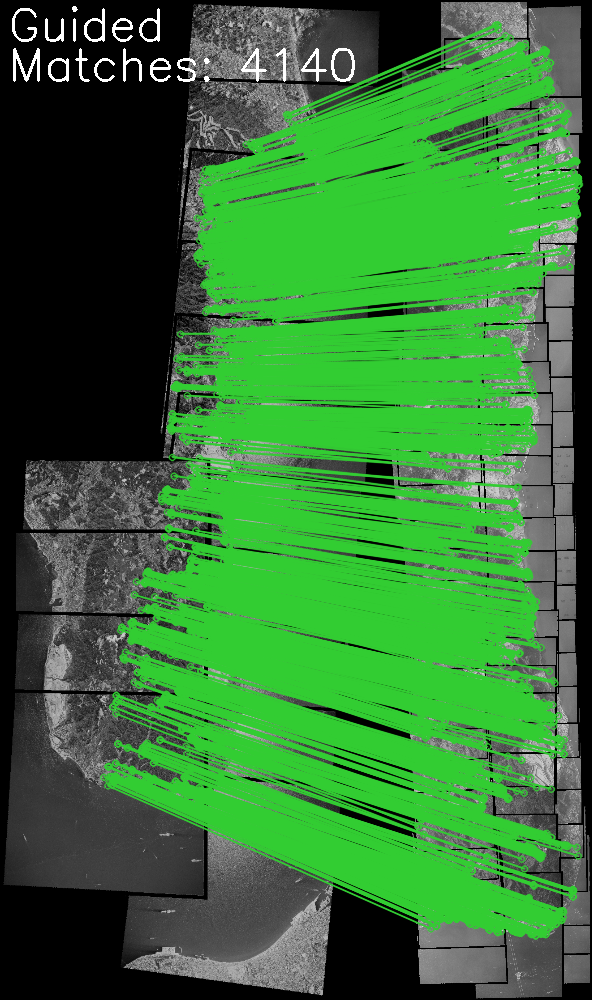
\includegraphics[width=3.8cm,angle=90]{images/Chapitre4/Precise-SpGDSMHomol-GuidedSIFT-3DRANSAC-CrossCorrelation-PileImg_Ortho-MEC-Malt_Tapas_1991_Ortho-MEC-Malt_Tapas_1994.png}
			\end{minipage}%
		}
		\subfigure[$Patch_{SIFTDSM}$]{
			\begin{minipage}[t]{0.48\linewidth}
				\centering
				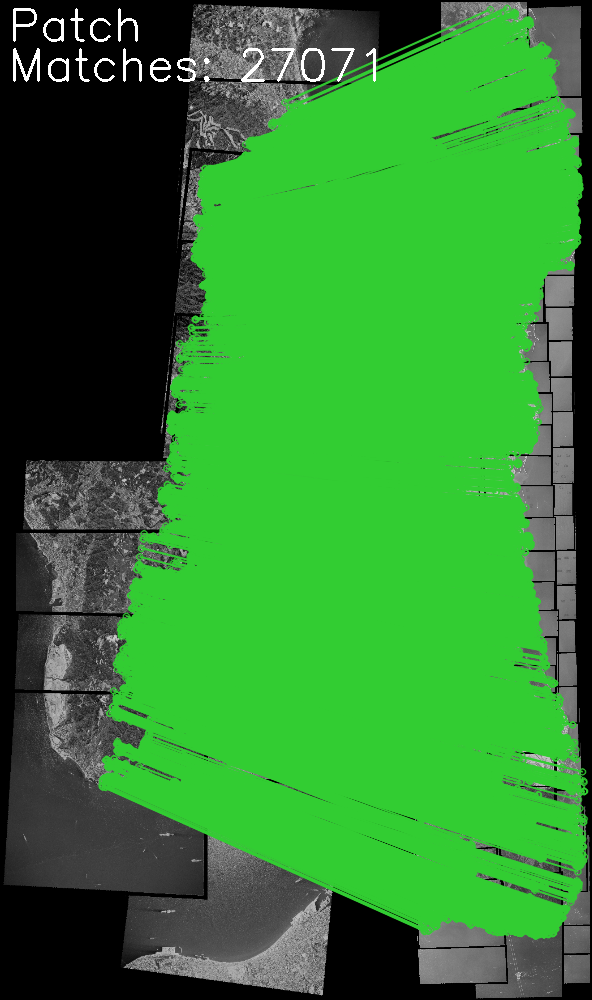
\includegraphics[width=3.8cm,angle=90]{images/Chapitre4/Precise-SIFTDSMHomol-SuperGlue-3DRANSAC-CrossCorrelation-PileImg_Ortho-MEC-Malt_Tapas_1991_Ortho-MEC-Malt_Tapas_1994.png}
			\end{minipage}%
		}
		\subfigure[$Guided_{SIFTDSM}$]{
			\begin{minipage}[t]{0.48\linewidth}
				\centering
				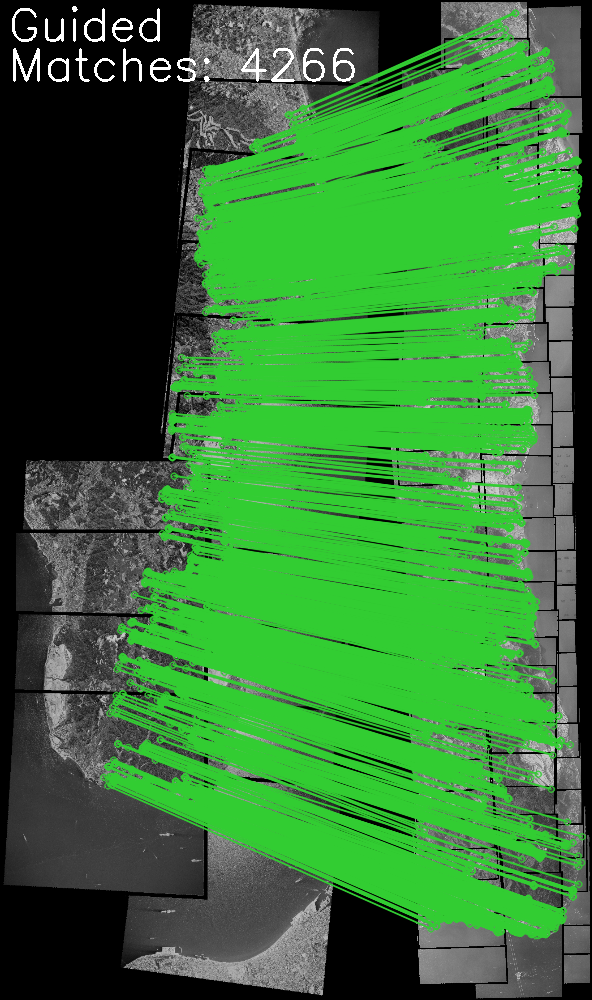
\includegraphics[width=3.8cm,angle=90]{images/Chapitre4/Precise-SIFTDSMHomol-GuidedSIFT-3DRANSAC-CrossCorrelation-PileImg_Ortho-MEC-Malt_Tapas_1991_Ortho-MEC-Malt_Tapas_1994.png}
			\end{minipage}%
		}
		\caption{Precise matching visualization of \textbf{Kobe 1991 and 1995}. (a) Image pairs to be matched, with red rectangles indicating the common zone. (b) Numbers of tentative, enhanced and final matches recovered with $Patch_{SpGDSM}$, $Guided_{SpGDSM}$, $Patch_{SIFTDSM}$ and $Guided_{SIFTDSM}$ individually. (c-f) Visualization of final matches recovered with $Patch_{SpGDSM}$, $Guided_{SpGDSM}$, $Patch_{SIFTDSM}$ and $Guided_{SIFTDSM}$ individually.}
		\label{MatchVizKobe}
	\end{center}
\end{figure*} 




